\documentclass[12pt]{article}
%\usepackage{report}

\usepackage[utf8]{inputenc} % allow utf-8 input
\usepackage[T1]{fontenc}    % use 8-bit T1 fonts
\usepackage[colorlinks=true, linkcolor=blue, citecolor=blue, urlcolor=blue]{hyperref}       % hyperlinks
\usepackage{url}            % simple URL typesetting
\usepackage{booktabs}       % professional-quality tables
\usepackage{amsfonts}       % blackboard math symbols
\usepackage{nicefrac}       % compact symbols for 1/2, etc.
%\usepackage{microtype}      % microtypography
\usepackage{lipsum}		% Can be removed after putting your text content
\usepackage{braket}
\usepackage{graphicx}
\usepackage{footnote}
\usepackage{doi}
\usepackage{comment}
\usepackage{multirow}
\usepackage{textcomp}
\usepackage{gensymb}
\usepackage{float}
\usepackage{amsmath}
\usepackage{subcaption}
\usepackage{setspace}
\usepackage[skip=10pt plus1pt, indent=30pt]{parskip}
\usepackage[top=1.5in, bottom=1.5in, left=1in, right=1in]{geometry}
\usepackage{titlesec}

\begin{document}
% Adjust section heading size
\titleformat{\section}{\large\bfseries}{\thesection}{0.5em}{}

% Adjust subsection heading size
\titleformat{\subsection}{\large\bfseries}{\thesubsection}{1em}{}

\begin{titlepage}
    \centering
    
\includegraphics[width=2.5cm]{crest.jpg}\par
    \vspace{0.5cm}
    {\scshape\Large Department of Physics and Astronomy \par}
    \vspace{0.25cm}
    {\scshape\Large The University of Southampton \par}
    \vspace{1cm}
    {\huge\bfseries Updates on the Inert Two Higgs Doublet Model (i2HDM) parameter space for Dark Matter discovery\par}
    \vspace{0.25cm}
    {\scshape\Large \bfseries Preliminary Report \par}
    \vspace{1cm}
    {\Large Ong Chin Phin (Linus) \par}
    \vspace{0.25cm}
    {\large Student ID: 33184747 \par}
    \vfill
    {\large Febuary 2025 \par}
\end{titlepage}

%\maketitle
%\newpage
%\tableofcontents
%\thispagestyle{empty}

\newpage
\thispagestyle{empty}

\begin{abstract}
The Higgs potential, characterized by a "Mexican hat" shaped function, determines the vacuum expectation value (VEV) of the Higgs boson, denoted as $v$. This potential leads to spontaneous symmetry breaking, where the Higgs field acquires a non-zero VEV, resulting in mass generation for certain particles.

Extending this framework, we explore the Inert Two-Higgs Doublet Model (i2HDM), which introduces a second Higgs doublet that is inert — meaning it does not acquire a VEV, does not couple to fermions, and preserves a discrete symmetry. This inert doublet contributes additional scalar particles, including a viable dark matter candidate, $h_1$.

In this study, we update the parameter space of the i2HDM, focusing on parameters such as the masses of the scalar particles ($m_{h_1}$, $m_{h_2}$, $m_{h_\pm}$), and the quartic couplings ($\lambda_2$, and $\lambda_{345}$).We incorporate the latest theoretical and experimental constraints. This preliminary report will include the current results and analysis done up to this point in the dissertation.
\end{abstract}

\section{Introduction and Theory}
Initially, the Universe was in a hot dense state with an unknown initial temperature. \footnote{As this was prior to the Big Bang, we don't know how hot it was. We know for sure it was above 10 MeV, otherwise the Big Bang would not happen. This should be sufficiently hot to generate protons and neutrons, allowing a process known as nucleosynthesis to happen, where new nuclei are created.} In this state, all particles were in thermal equilibrium within a plasma. Then 14 billion years ago, the Big Bang occurred - an expansion from a singularity which slowed down over time due to inflation.

We assume that if DM is a particle, then at high temperatures, it behaved relativistically like other particles. However, as the universe cooled down exponentially, there was a point where the temperature of the universe dropped below the mass of DM. This led to DM annihilation with standard model (SM) particles, an irreversible process which lowered the density of DM particles. 

The annihilation rate, which depends on the interaction cross section determined how much DM remained (the relic density). An annihilation process that is too efficient would lead to too low relic density, which would not pose too much of a problem. However, a relic density that is too high will cause an unstable Universe and cause it to collapse on itself. The reality is that DM particles eventually stopped interacting with SM particles, leading to a process known as freeze out, giving a constant relic density. This process can be described via the Boltzmann equation.

\subsection{Inert Two Higgs Doublet Model (i2HDM)}
\label{sec:i2HDM}
In the i2HDM, we propose two doublets, $\Phi_1$, $\Phi_2$ - where the first doublet is active and second doublet is inert. The latter does not share its degrees of freedom with other particles (or, it does not couple to fermions via Yukawa interactions \cite{Belyaev_2022}), and has no VEV; unlike the former which is just the SM Higgs doublet, which has a VEV. We can invoke a new set of particles arising from $\Phi_2$- $h^\pm, h_1,$ and $h_2$, where $m_{h_1} < m_{h_2}$ and $m_{h_1} < m_{h^\pm}$. The lightest particle, $h_1$ is the DM candidate particle.

As mentioned in the Introduction (Section \ref{sec:introduction}), i2HDM is an extension of SM that introduces new scalar particles that could be candidates for DM.

The field, along with its Hermitian conjugate is:
\begin{align}
    &\Phi_2 = \frac{1}{\sqrt{2}}
        \begin{pmatrix}
            {\sqrt{2}h^+} \\
            {h_1 + ih_2 }
        \end{pmatrix}&
    &\Phi_2^\dagger = \frac{1}{\sqrt{2}} 
        \begin{pmatrix}
            {\sqrt{2}h^-} \\
            {h_1 - ih_2 }
        \end{pmatrix}
\end{align} 

The (scalar) potential is expressed as:
\begin{equation}
    \begin{split}
        V(\Phi_1, \Phi_2) =& -m_1^2(\Phi_1^\dagger\Phi_1) - m_2^2(\Phi_2^\dagger\Phi_2)\\ 
        &+ \lambda_1(\Phi_1^\dagger\Phi_1)^2 + \lambda_2(\Phi_2^\dagger\Phi_2)^2 \\
        &+ \lambda_3(\Phi_1^\dagger\Phi_1)(\Phi_2^\dagger\Phi_2) \\
        &+ \lambda_4(\Phi_2^\dagger\Phi_1)(\Phi_1^\dagger\Phi_2)\\ 
        &+ \frac{\lambda_5}{2}[(\Phi_1^\dagger\Phi_2)^2 + (\Phi_2^\dagger\Phi_1)^2]
        \end{split}
        \label{eq:higgs_potential}
\end{equation}

Where:
\begin{itemize}
    \item $\Phi_1$ represents the active doublet
    \item $\Phi_2$ represents the inert doublet
    \item $m_1$ is the term which determines the mass of the Higgs boson and symmetry breaking\footnote{The negative sign in the first term of Equation \ref{eq:higgs_potential} makes the first term a potential with negative slope, which introduces spontaneous symmetry breaking and gives the active Higgs doublet the VEV.}
    \item $m_2$ is the mass term of the inert Higgs doublet (which helps determine the masses of the extra particles, $h_1$, $h_2$ and $h_\pm$)
    \item $\lambda_{1, 2}$ are self coupling terms of the doublets. $\lambda_1$ determines the mass of the Higgs boson and $\lambda_2$ determine the 
    \item $\lambda_{3, 4, 5}$ are the coupling terms of doublet interaction
\end{itemize}
Furthermore, we impose additional parametrisation in terms of mass differences that allow better visualisation of parameter space \cite{Belyaev_2022}, the reason which will be prevalent in the next sections when considering constrains:
\begin{align}
\label{eq:mass_diff_1}
    \Delta m^{0} = m_{h_2} - m_{h^\pm},\\
    \Delta m^1 = m_{h_2} - m_{h_1},\\
    \Delta m^+ = m_{h^\pm} - m_{h_1}
\end{align}

\subsection{Constraints of the i2HDM}
We have four parameters to scan across: $m_{h_1}$, $\Delta m^0$, $\Delta m^+$ and $\lambda_{345}$ ($\lambda_3 + \lambda_4 + \lambda_5$), with $\lambda_2 = 1$. We can set $\lambda_2 = 1$ because $\lambda_2$ does not affect DM phenomenology at the tree level\footnote{lowest-order approximation in perturbation theory, where Feynman diagrams do not include loops (closed paths)}\cite{Belyaev:2016lok}; it only governs self interaction of the inert Higgs doublet, does not affect physical observables, and the DM candidate $h_1$ is only dependent on $\lambda_3$, $\lambda_4$ and $\lambda_5$ (Equation \ref{eqn:massdmscalar}). While $\lambda_2$ does not appear explicitly in the relevant interactions, it indirectly contributes to vacuum stability, ensuring a consistent and physically viable model. Setting $\lambda_2 = 1$ also greatly reduces computing load and time. The masses of $h_2$, $h_\pm$ are then calculated using Eqn. \ref{eq:mass_diff_1}.

This will be a random scan of the parameter space, done with the software \verb|microOMEGAS|, version 6.1.15. Through theory and experiments, there are certain constraints that will have to be applied to the scan such that a proper search can be done.

\subsubsection{Constraints from vacuum permeability}
First of all, we need to ensure that the potential is bounded from below to ensure stability \cite{Deshpande:1977rw}:
\begin{equation}
    \begin{split}
    \lambda_1>0,& \qquad
    \lambda_2>0, \qquad
    \lambda_3> -2 \sqrt{ \lambda_1 \lambda_2}, \\
    &\lambda_3 + \lambda_4 - |\lambda_5| > -2 \sqrt{ \lambda_1 \lambda_2}.
    \end{split}
    \label{eq:potential_stability}
\end{equation}
We can describe the parameter space of the i2HDM as \cite{Belyaev:2016lok}:
\begin{equation}
    \begin{split}
        m_{h_1}, \qquad m_{h_2} > m_{h_1}, \qquad m_{h^\pm} > m_{h_1}, \\
        \lambda_2 > 0, \qquad \lambda_{345} > -2\sqrt{\lambda_1 \lambda_2}
    \end{split}
\end{equation}

Where $m_{h_1}$, $m_{h_2}$ and $m_{h^\pm}$ are the masses of the 2 neutral and 2 charged inert scalars. This is to ensure that the Higgs potential is bounded from below and has a neutral, non-charge breaking vacuum, which is only satisfied if:
\begin{equation}
    \lambda_4 - |\lambda_5| < 0
\end{equation}

One could evaluate the masses of these physical scalars \cite{Belyaev:2016lok}:
\begin{align}
    \label{eqn:scalar_equations}
    &m_{Higgs}^2 = 2\lambda_1v^2 = 2m^2_1,\\
    &m_{h_\pm} = \frac{1}{2}\lambda_3v^2-m^2_2 \\
    \label{eqn:massdmscalar}
    &m_{h_1}^2 = \frac{1}{2}(\lambda_3 + \lambda_4 - |\lambda_5|)v^2 - m_2^2\\
    &m_{h_2}^2 = \frac{1}{2}(\lambda_3 + \lambda_4 + |\lambda_5|)v^2 - m_2^2 > m^2_{h_1}
\end{align}

and the mass differences: 
\begin{align}
    &m_{h_2}^2 - m_{h_1}^2 =  |\lambda_5|v^2, \\
    &m_{h_\pm}^2 - m_{h_2}^2 = -\frac{1}{2}(\lambda_4 - |\lambda_5|)v^2
\end{align}

$m_{h_1}$, $m_{h_2}$, $m_{h_\pm}$ and $\lambda_{345}$ are the main parameters of the study. $\lambda_{345}$ is an important parameter as it is involved in the $H\rightarrow h_1,h_1$ and $h_1,h_1 \rightarrow H$ (written in short as $Hh_1h_1$) interaction vertex. $\lambda_1$ is not a free parameter due to the reasons discussed earlier.

In addition to that, we consider constraints due to symmetry breaking. We impose that, from \cite{Belyaev:2016lok, Ginzburg2010}:

\begin{equation}
    m_{h_1}^2 >
        \begin{cases}
         0, & |R| < 1\\
         (R-1) \sqrt{\lambda_1\lambda_2} v^2, & R>1
        \end{cases}
\end{equation}

Where:
\begin{equation}
    R = \frac{\lambda_{345}}{2\sqrt{\lambda_1\lambda_2}}
\end{equation}
$\lambda_1$, the self coupling term for the Higgs boson can be evaluated (from Equation \ref{eqn:scalar_equations}):
\begin{equation}
    \begin{split}
        \lambda_1 &= \frac{m^2_{Higgs}}{2 v^2}
                \approx\frac{125^2}{2\cdot 246 ^ 2} \\
                &\approx0.129
    \end{split}
\end{equation}

In addition, we can see from equation \ref{eqn:R>1} this can be rewritten as:
\begin{equation}
    \lambda_{345} < 2\left( \frac{m_{h_1}^2}{v^2} + \sqrt{\lambda_1\lambda_2}\right)
\end{equation}

\subsubsection{Constraints form perturbativity and unitarity}
As shown in 



\subsubsection{Constraints from LEP and EWPT (Electroweak Precision Data)}
From LEP, we can see that the constraints follow the W and Z boson widths:
\begin{align}
    m_{h_1} + m_{h_\pm} > m_{W^\pm}, \qquad
    m_{h_2} + m_{h_\pm} > m_{W^\pm}, \qquad  \label{LEP2_1}
    \\
    m_{h_1} + m_{h_\pm} > m_{Z^0}, \qquad
    2m_{h_\pm} > m_{Z^0}, \qquad  \label{LEP2_2}
\end{align}

From LEP II \cite{Lundstr_m_2009}, there are the additional constraints on the masses and mass differences:
\begin{align}
    m_{h_1}< 80 \text{ GeV}, \qquad
    m_{h_2}< 100 \text{ GeV}, \qquad \label{LEP2_3}
    \\
    m_{h_2} - m_{h_1} > 8\text{ GeV}, \qquad
    m_{h_\pm}> 70\text{ GeV} \qquad \label{LEP2_4}
\end{align}

From \cite{gfitter2014global}, for a Higgs boson mass of 125 GeV, we have values for $S$, $T$ and $U$, the Peskin-Takeuchi parameters \cite{PeskinTakeuchi1990} which describe potential new physics contributions (for example - BSM) to electroweak radiative corrections.

 The values for $S$ and $T$ when setting $U = 0$ are:
 \begin{align}
     S = 0.06 \pm0.09, \qquad
     T = 0.10\pm0.07
 \end{align}

With a correlation coefficient of $+0.91$. Setting $U = 0$ allows simplification in parameter space, requiring only focus on the $S-T$ plane, which are more dominant. Defining:
\begin{align}
    x_1 = \frac{m_{h_1}}{m_{h_\pm}}, \qquad 
    x_2 = \frac{m_{h_2}}{m_{h_\pm}}
\end{align}
As well as:
\begin{align}
    &f_a(x) = -5 +12\log(x), \qquad
    f_b(x) = 3-4\log(x),
    \\
    &f_c(x,y) = 
    \begin{cases}
        \frac{x+y}{2}-\frac{xy}{x-y}\log{\left(\frac{x}{y}\right)}, & x\neq y\\
        0, & x = y
    \end{cases}
\end{align}

The S and T parameters are given with the equation:
\begin{align}
    &S = \frac{1}{72\pi}\frac{1}{(x^2_2 - x^2_1)^3}[x^6_2f_a(x_2)-x^6_1f_a(x_1) + 9x_2^2x_1^2(x_2^2f_b(x_2)-x^2_1f_b(x_1)] \label{eqn:S}
    \\
    &T = \frac{1}{32\pi^2\alpha\nu}[f_c(m^2_{h_\pm},m^2_{h_2}) + f_c(m^2_{h_\pm},m^2_{h_1}) - f_c(m^2_{h_2},m^2_{h_1})] \label{eqn:T}
\end{align}

\subsubsection{Constraint from Dark Matter Relic Density}
\label{sec:relic density}
DM relic density is the remaining DM from the Big Bang, and there are multiple experiments (PLANCK, WMAP) that calculate various cosmological parameters, one of them being the DM relic density. We can use this very accurate data to limit our parameter space to make the search for DM simpler. The latest experimental value for DM relic density is  \cite{Planck:2018vyg}:
\begin{equation}
    \Omega ^{PLANCK}_{DM} h^2 = 0.11933 \pm 0.00091
\end{equation}

We set the parameter space for the density of the DM relic to ignore the cases of DM overabundance (where $\Omega h^2 > \Omega^{PLANCK}_{DM_{max}}h^2$). DM overabundance is not considered as it leads to inconsistencies with the observed CMB and its constraints \cite{Croon_2024, Zavala_2010}. DM under-abundance is allowed to allow for possible external sources of DM.

For data interpretation purposes, and since \verb|micrOMEGAS| software calculates relic density via tree-level calculation, the theoretical constraints applied to the density of DM relics will be within $\pm10\%$ of the value of $\Omega ^{PLANCK}_{DM} h^2$.
\begin{equation}
    \begin{split}
        \Omega_{DM} h^2 &= 0.11933 \pm 10\% \\
        &\approx 0.119 \pm 0.012
    \end{split}
    \label{eqn:DM relic density value}
\end{equation}

\subsubsection{Constraints from DM Direct Detection (DD), CMB and Branching Ratios}
The constraints applied from DM DD experiments are applied via a p-value. A p-value of 0.1 is used, and values greater than 0.1 are accepted to exclude values given by DD experiments.

There also is the chance that the values obtained could have been excluded by the CMB. CMB measurements are sensitive to energy injections in the early universe, such as those from dark matter annihilations. Ensuring that the model complies with CMB constraints helps in maintaining consistency with observed cosmological parameters. 

The upper limit of the branching ratio for the invisible Higgs at 95\% confidence level from the latest ATLAS search is\cite{ATLAS:2022yvh}:
\begin{equation}
    Br(\text{Higgs} \rightarrow \text{invisible}) = 0.145
\end{equation}


\section{Preliminary Results and Analysis}
A 5-D scan is done across the parameters stated earlier and by applying "cuts" to the 5-D datasets, we can then narrow the parameter space in our search for the DM particle.
We apply cuts in the following order:
\begin{itemize}
    \item Cut 1 - Constraints from vacuum permeability and stability (Eqn. \ref{eqn:R>1})
    \item Cut 2 - Constraints from LEP (Eqn. \ref{LEP2_1}, \ref{LEP2_2}, \ref{LEP2_3}, \ref{LEP2_4}) and EWPT (Eqn. \ref{eqn:S}, \ref{eqn:T})
    \item Cut 3 - Constraint from the experimental value of DM relic density (Eqn. \ref{eqn:DM relic density value}) - also adding an option for a "strict" bound - a $\pm 10 \%$ bound on the value of relic density.
    \item Cut 4 - Constraints from DM direct detection, CMB data and branching ratios.
\end{itemize}

The 5-D datasets are projected onto a 2-D plane, and majority of the plots can be found in the \hyperref[sec:Appendix]{Appendix}.

\subsection{2-D Projection}
We can first consider the relationship between $m_{h_1}$ and $\lambda_{345}$. 
\begin{figure}
    \centering
    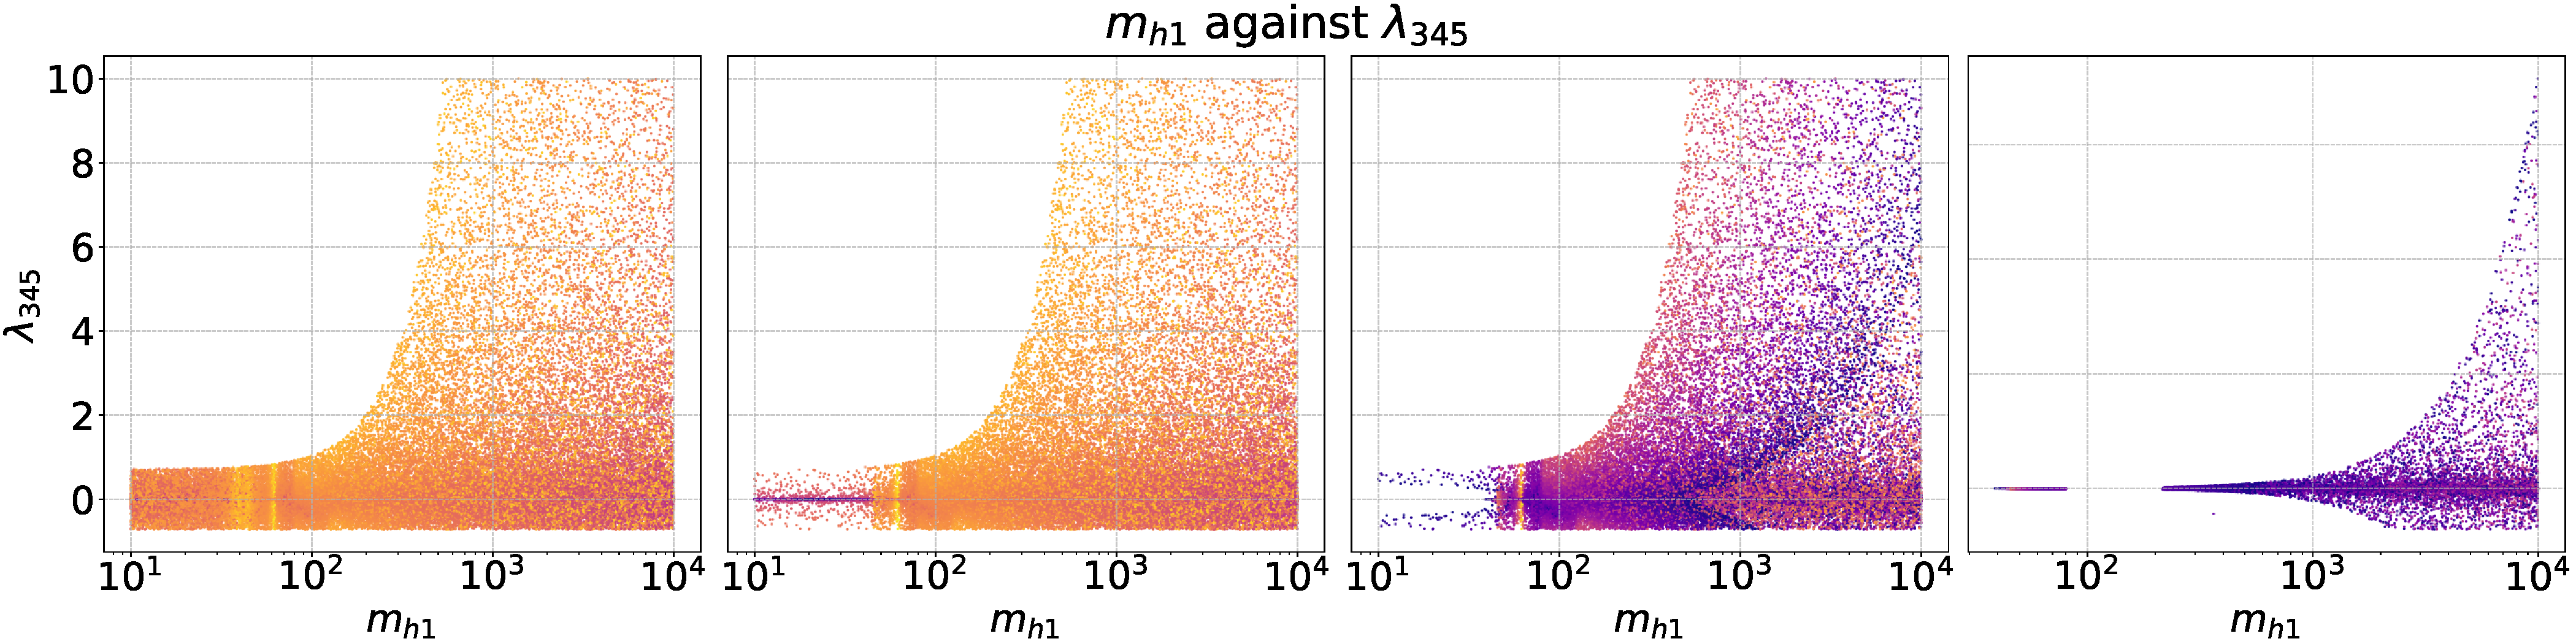
\includegraphics[width=\linewidth]{4plot/MD1_l345.pdf}
    \caption{Plot of $\lambda_{345}$ against $m_{h_1}$, coloured by $\Omega h^2$. From left to right are Cuts 1-4 applied onto the data. }
    \label{fig:enter-label}
\end{figure}

\subsection{1-D Analysis}
\label{1-D scan}
We can investigate the affect of $\lambda_{345}$ on $\Omega h^2$ (Fig. \ref{fig:MD1_l345_1}, \ref{fig:MD1_l345_100}) as done in \cite{Belyaev:2016lok}:
\begin{figure}[H]
    \centering
    \begin{subfigure}[b]{0.49\textwidth}
        \centering
        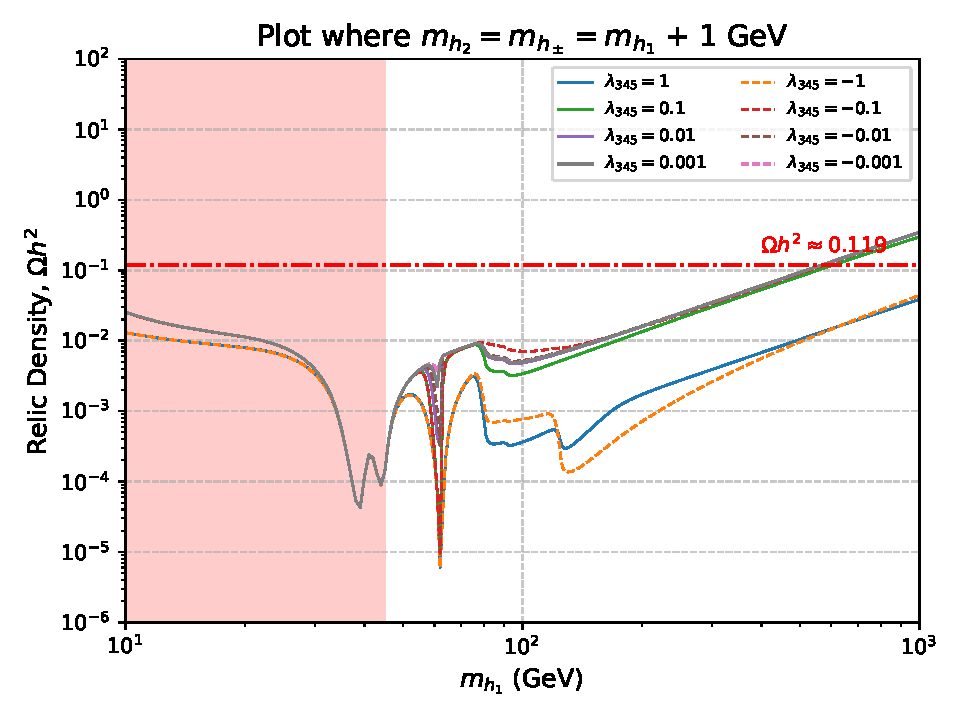
\includegraphics[width=\textwidth]{plots/plot_MD1_l345+1.pdf}
        \caption{Relic density against $m_{h_1}$, the case where $\Delta m^0 = 1$ GeV.}
        \label{fig:MD1_l345_1}
    \end{subfigure}
    \hfill
    \begin{subfigure}[b]{0.49\textwidth}
        \centering
        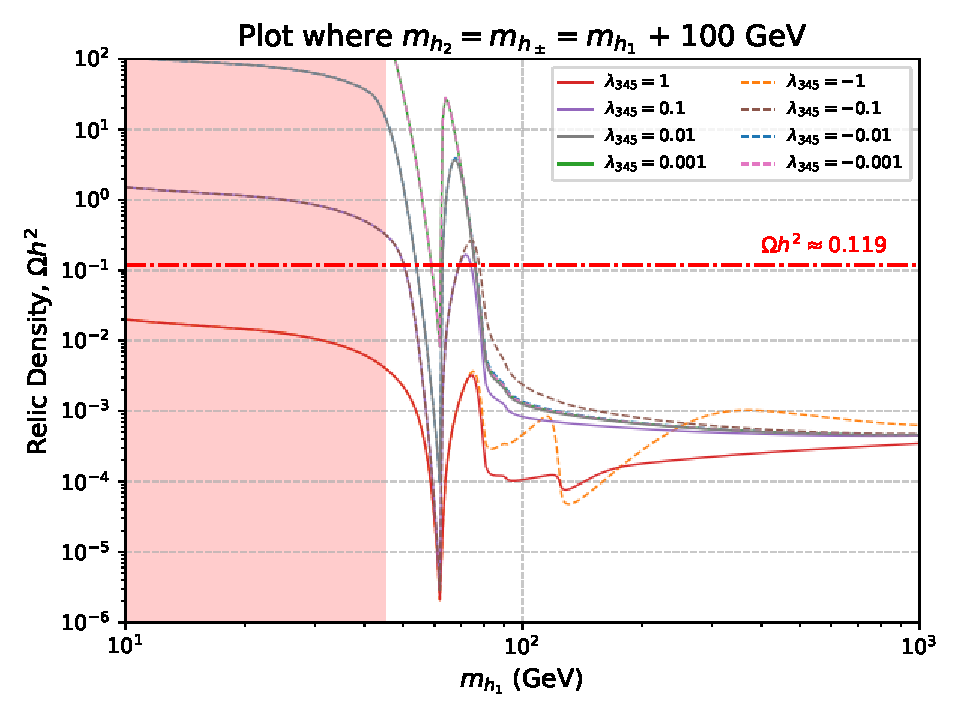
\includegraphics[width=\textwidth]{plots/plot_MD1_l345+100.pdf}
        \caption{Relic density against $m_{h_1}$, the case where $\Delta m^0 = 100$ GeV.}
        \label{fig:MD1_l345_100}
    \end{subfigure}
    \caption{Plots of relic density against $m_{h_1}$ for different mass differences (while keeping $m_{h_1}$ lightest). The red shaded region is the area excluded by LEP, and the red line the upper limit of DM relic density (Eqn. \ref{eqn:DM relic density value}).}
\end{figure}

In Fig. \ref{fig:MD1_l345_1} and \ref{fig:MD1_l345_100}, we alter the masses of the DM candidate, $h_1$ and its complementary particles ($h_2$ and $h_{\pm}$) to observe the relic density, we make a few observations:
\begin{itemize}
    \item The slight dips at 40 and 45 GeV for all values of $\lambda$ is the decay channel where $h_1, h_2 \rightarrow Z_0$ boson, and also the reaction for $h_1, h_{\pm} \rightarrow W_\pm$. The $Z^0$ and $W^\pm$ boson have masses $\sim$80 GeV and $\sim$85 GeV respectively.
    \item At $\sim$60 GeV, there is a dip for all values of $\lambda$ - this is because that is the $h_1,h_1\rightarrow H$ process - the DM DM decay process. 
    \item At 80-90 GeV, we can observe a slight dip for relic density for all values of $\lambda$ except for $\lambda = \pm1$. The reason this happens is because that is the annihilation channel for $h, h \rightarrow Z_0Z_0$ and $h, h \rightarrow W_+ W_-$.
    \item At $\sim$120 GeV, there is no obvious change in relic density except for $\lambda = \pm1$. This is the $h_1,h_1\rightarrow H H$ annihilation channel, which takes place only for big values of $\lambda_{345}$ due to stronger coupling term.
\end{itemize}

\section{Further Work}
For the remainder of the project, the cross sections of DM annihilation processes will be investigated. 
\newpage
\bibliographystyle{plain}
\bibliography{Documents/Thesis/references}

\newpage
\section{Appendix}
\label{sec:Appendix}
The remaining plots mentioned in Section \ref{5-D scan} are shown below, with cuts applied from left to right in the following order: Cut 1, Cut 1 and 2, Cut 1, 2 and 3, and Cut 1, 2, 3 and 4:
\begin{figure}[H]
    \begin{subfigure}[b]{\columnwidth}
      \centering
      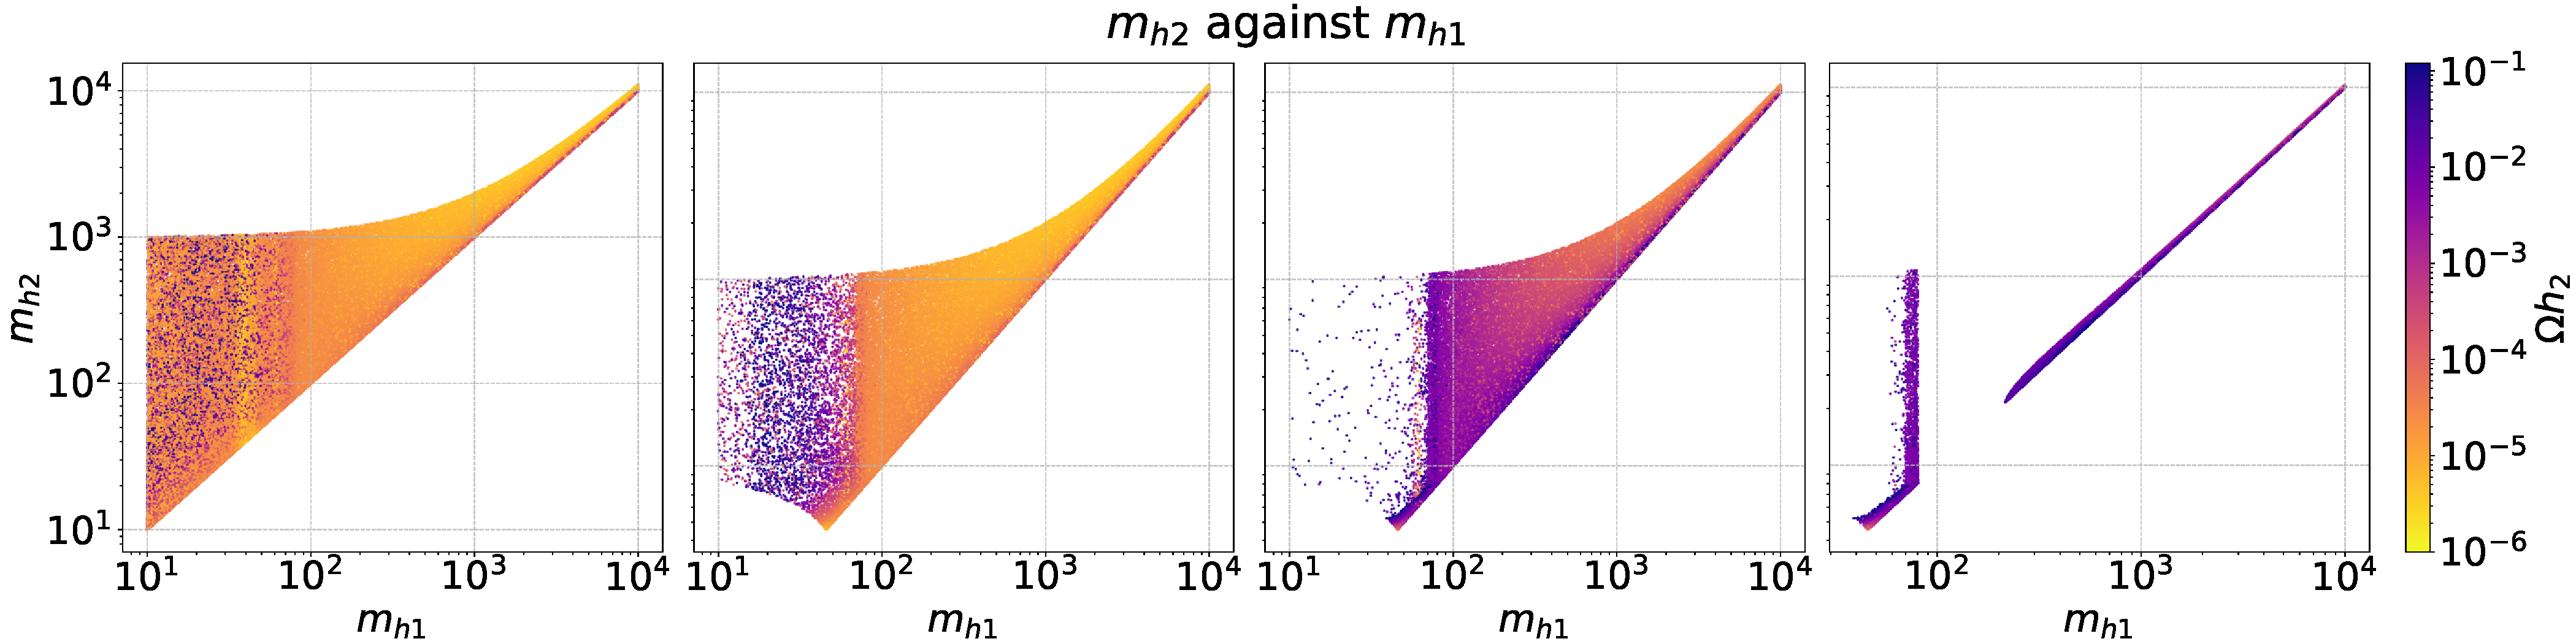
\includegraphics[width=1\columnwidth]{4plot/MD1_MD2.pdf}
    \end{subfigure}

    \begin{subfigure}[b]{\columnwidth}
      \centering
      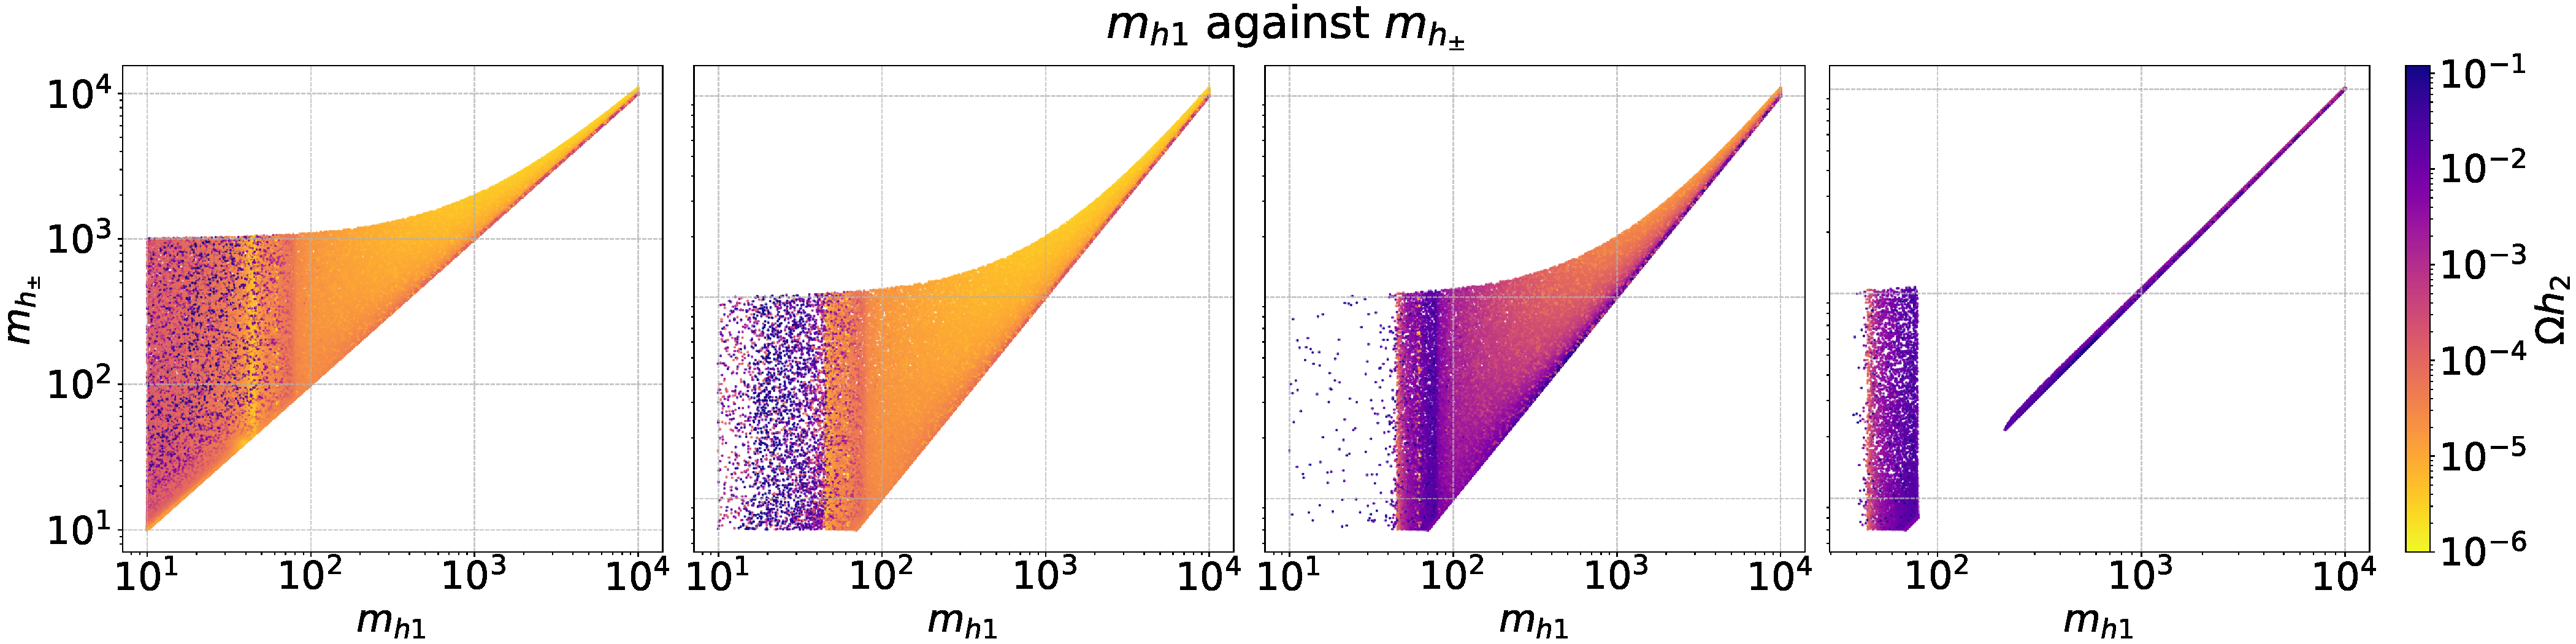
\includegraphics[width=1\columnwidth]{4plot/MD1_MDP.pdf}
    \end{subfigure}
    \caption{Plots of $m_{h_1}$ against other masses. From left to right: Constraints from vacuum permeability; constraints from LEP and EWPT; constraints from DM relic density; constraints from DM DD and CMB data.}
\end{figure}

\begin{figure}[H]
    \begin{subfigure}[b]{\columnwidth}
      \centering
      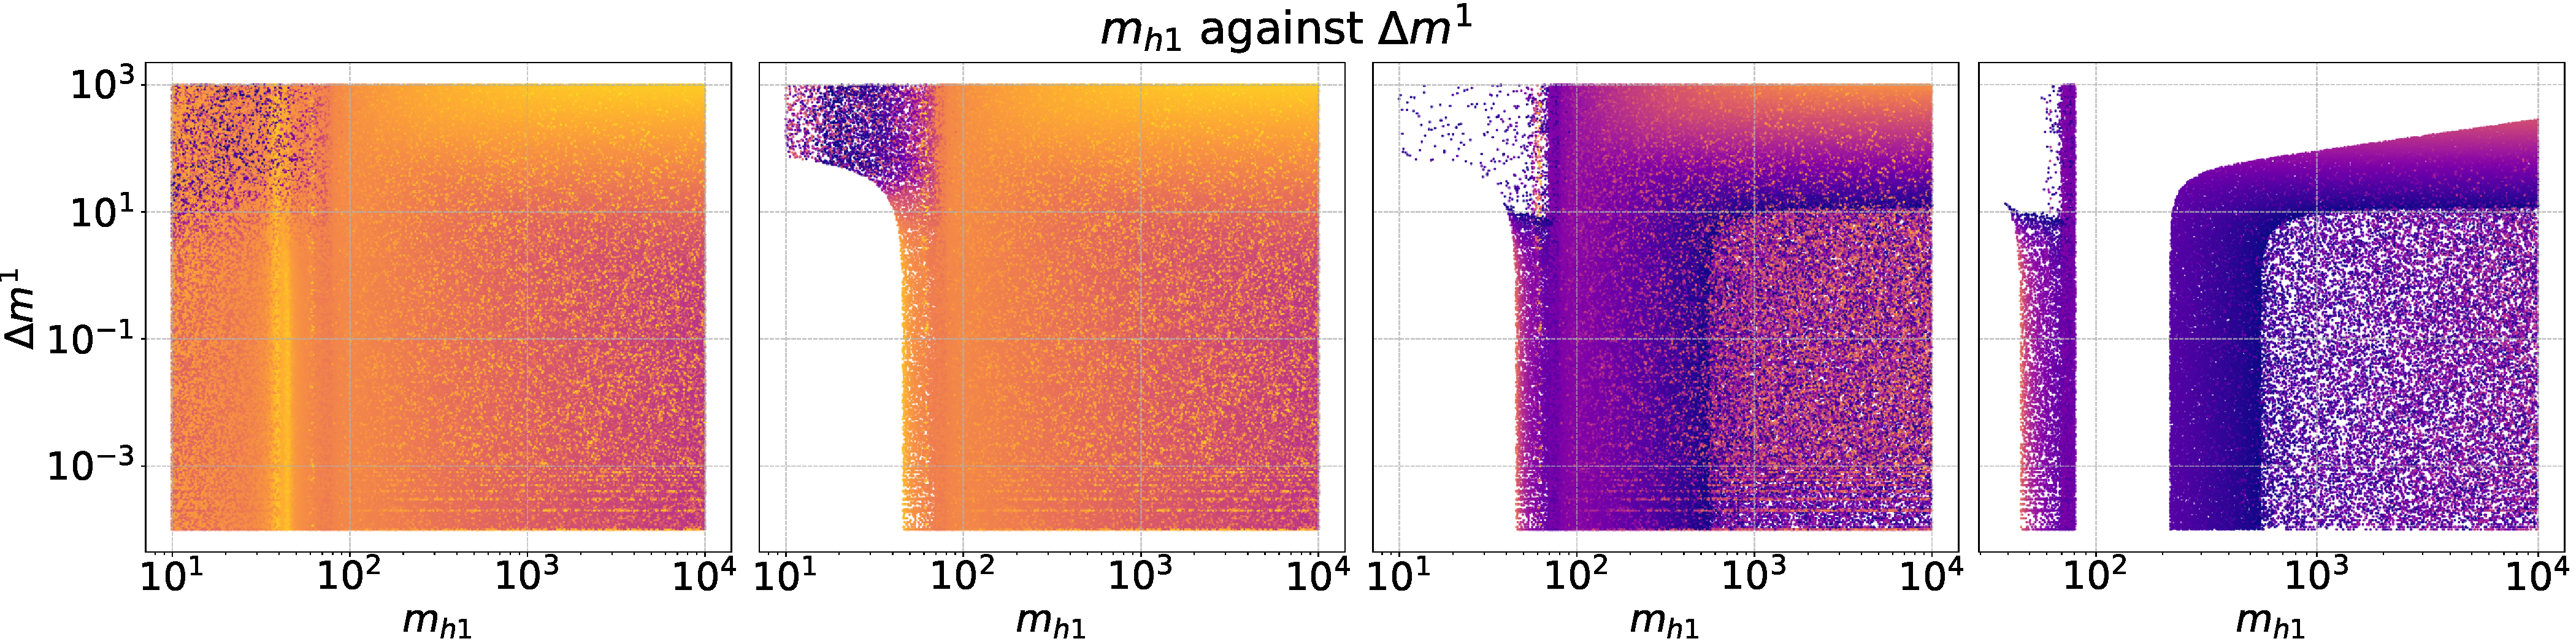
\includegraphics[width=1\columnwidth]{4plot/MD1_DM2.pdf}
    \end{subfigure}
    
    \begin{subfigure}[b]{\columnwidth}
      \centering
      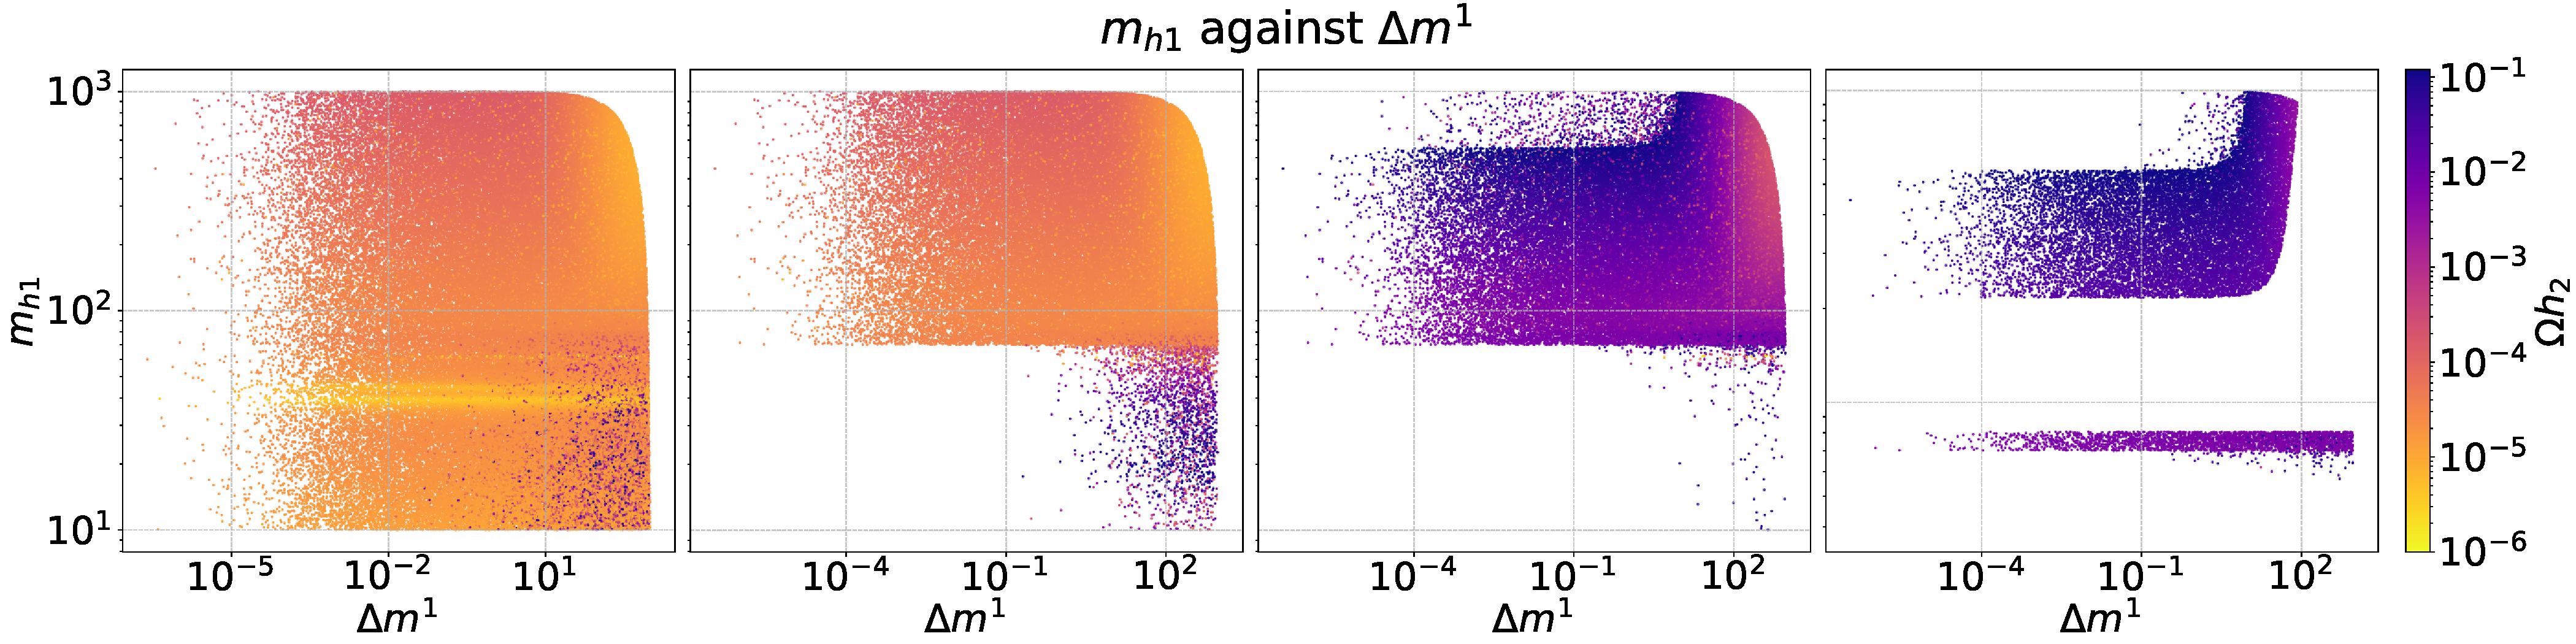
\includegraphics[width=1\columnwidth]{4plot/MD1_DM3.pdf}
    \end{subfigure}

    \begin{subfigure}[b]{\columnwidth}
      \centering
      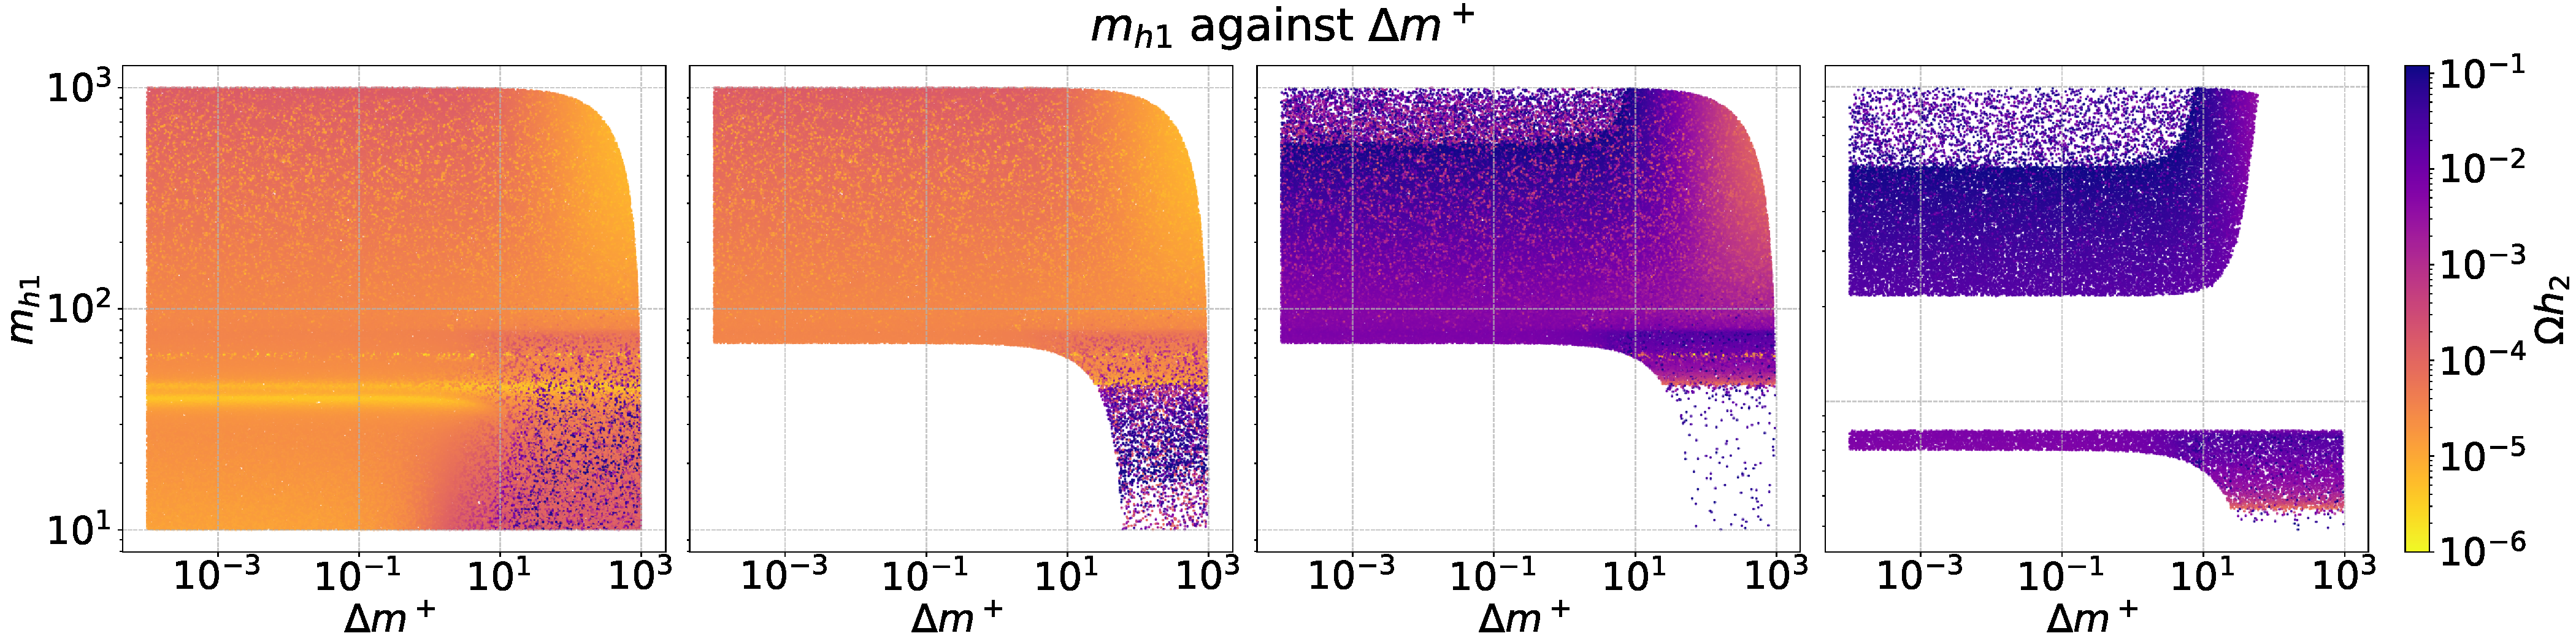
\includegraphics[width=1\columnwidth]{4plot/MD1_DMP.pdf}
    \end{subfigure}
    \caption{Plots with $m_{h1}$ against mass differences.}
\end{figure}


\begin{figure}[H]
    \begin{subfigure}[b]{\columnwidth}
      \centering
      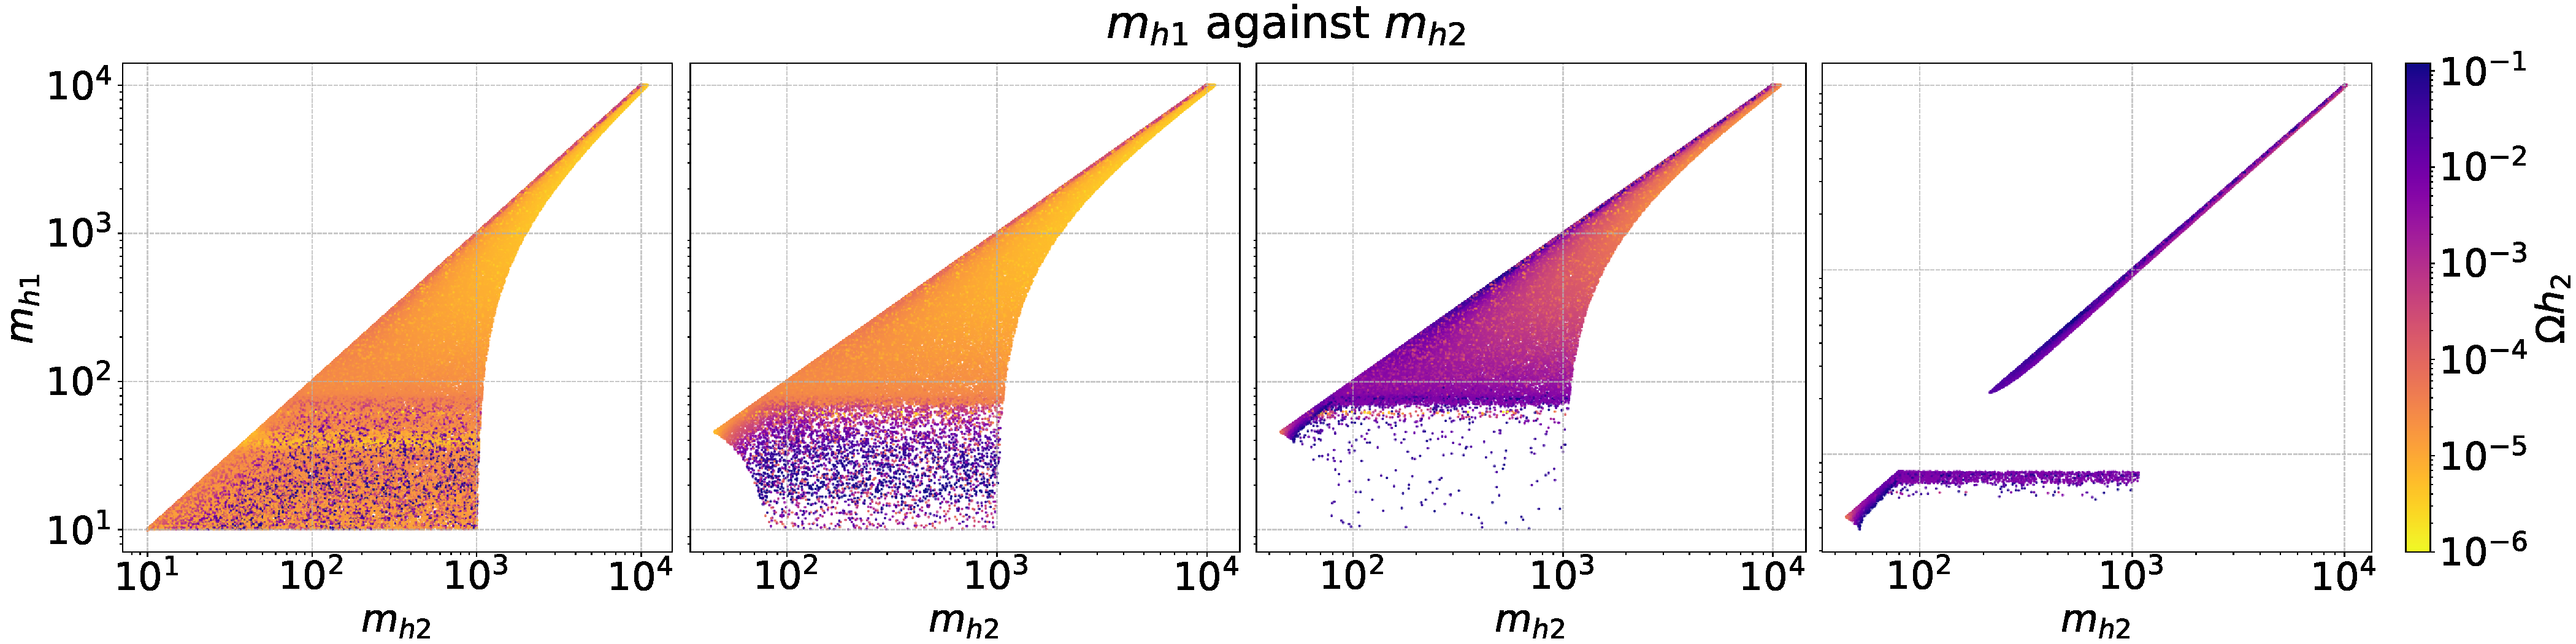
\includegraphics[width=1\columnwidth]{4plot/MD2_MD1.pdf}
    \end{subfigure}

    \begin{subfigure}[b]{\columnwidth}
      \centering
      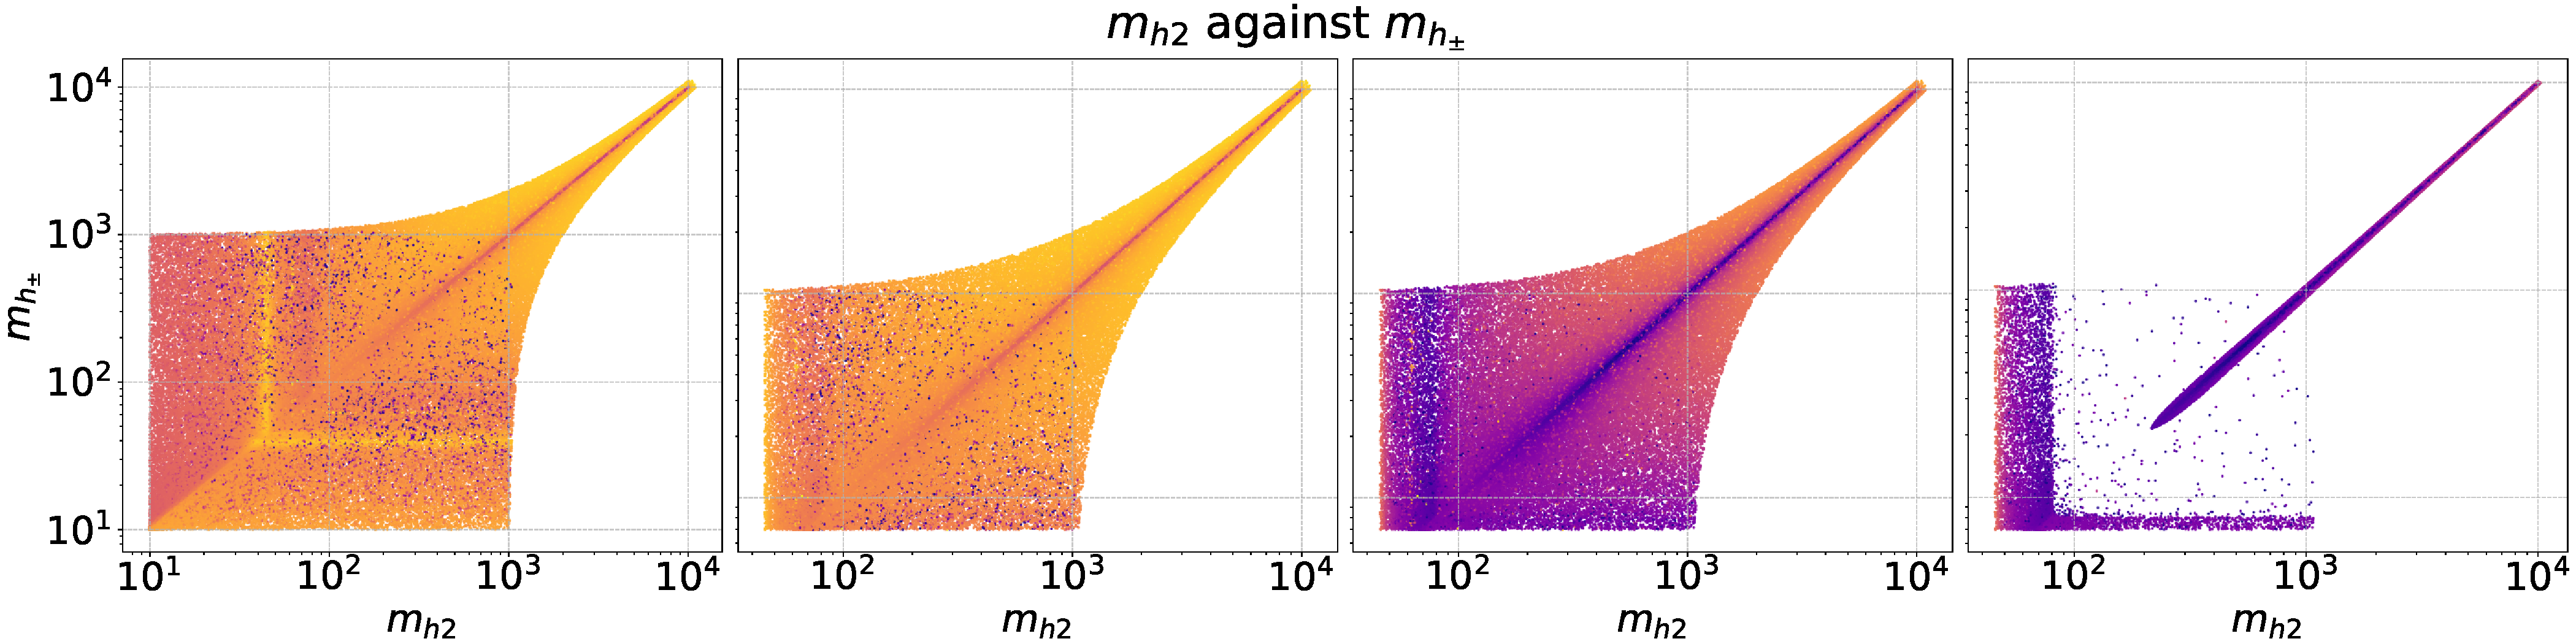
\includegraphics[width=1\columnwidth]{4plot/MD2_MDP.pdf}
    \end{subfigure}
    \caption{Plots of $m_{h_1}$ against other masses.}
\end{figure}

\begin{figure}[H]
    \begin{subfigure}[b]{\columnwidth}
      \centering
      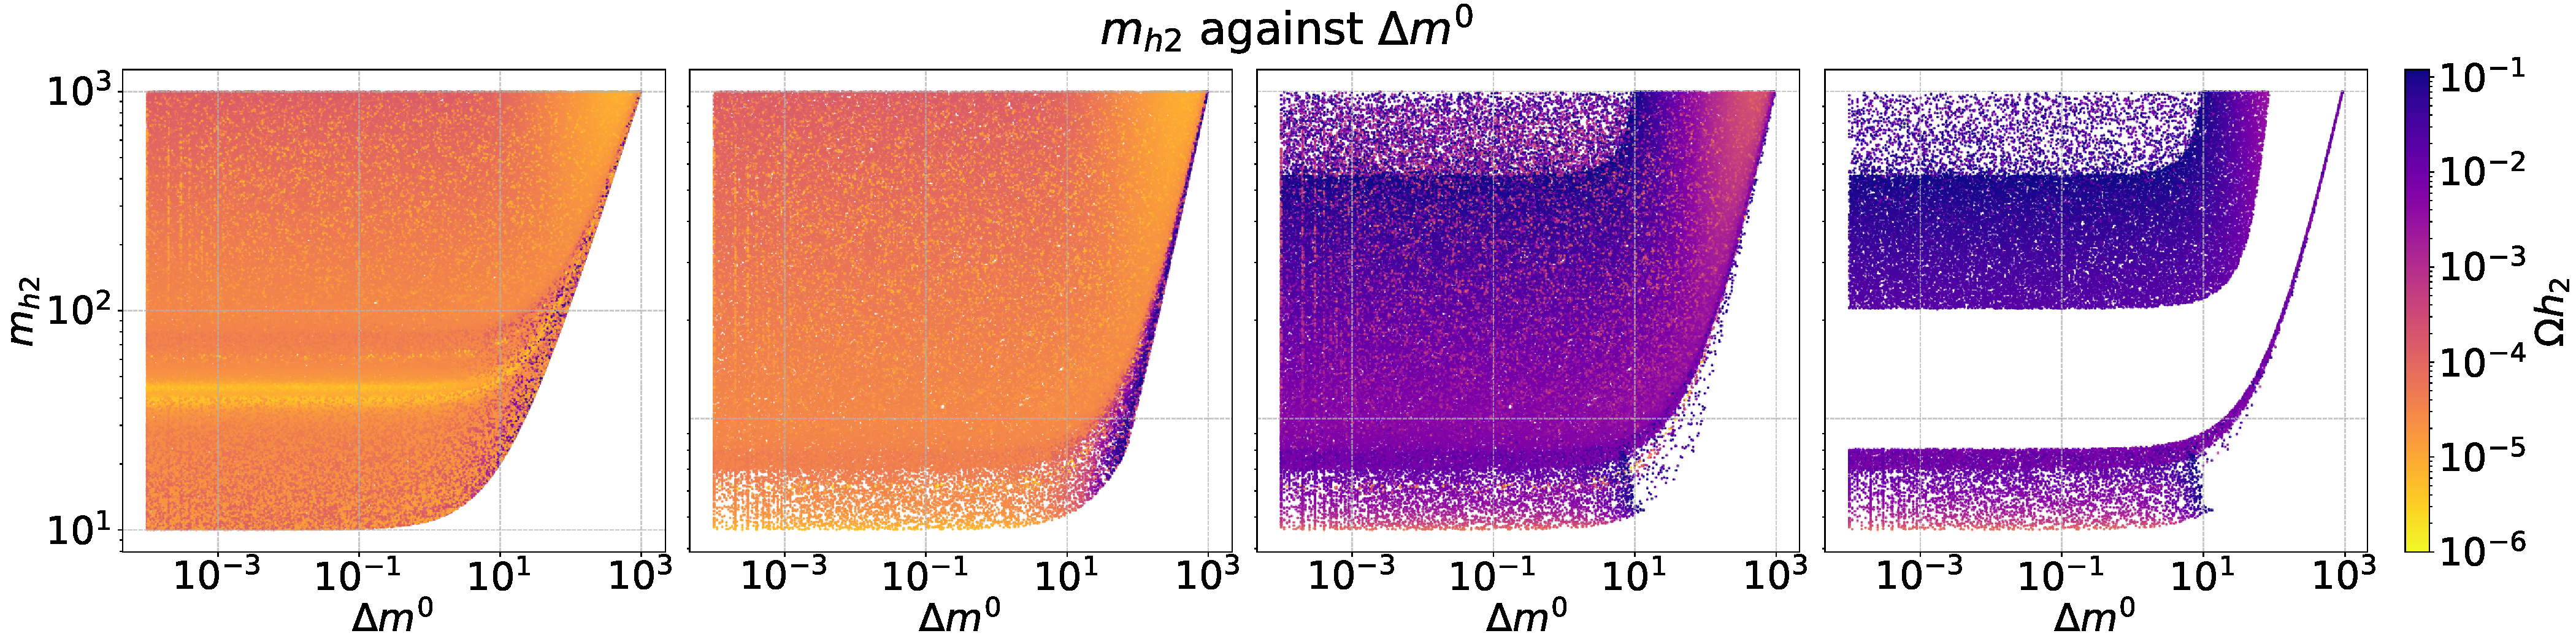
\includegraphics[width=1\columnwidth]{4plot/MD2_DM2.pdf}
    \end{subfigure}
    
    \begin{subfigure}[b]{\columnwidth}
      \centering
      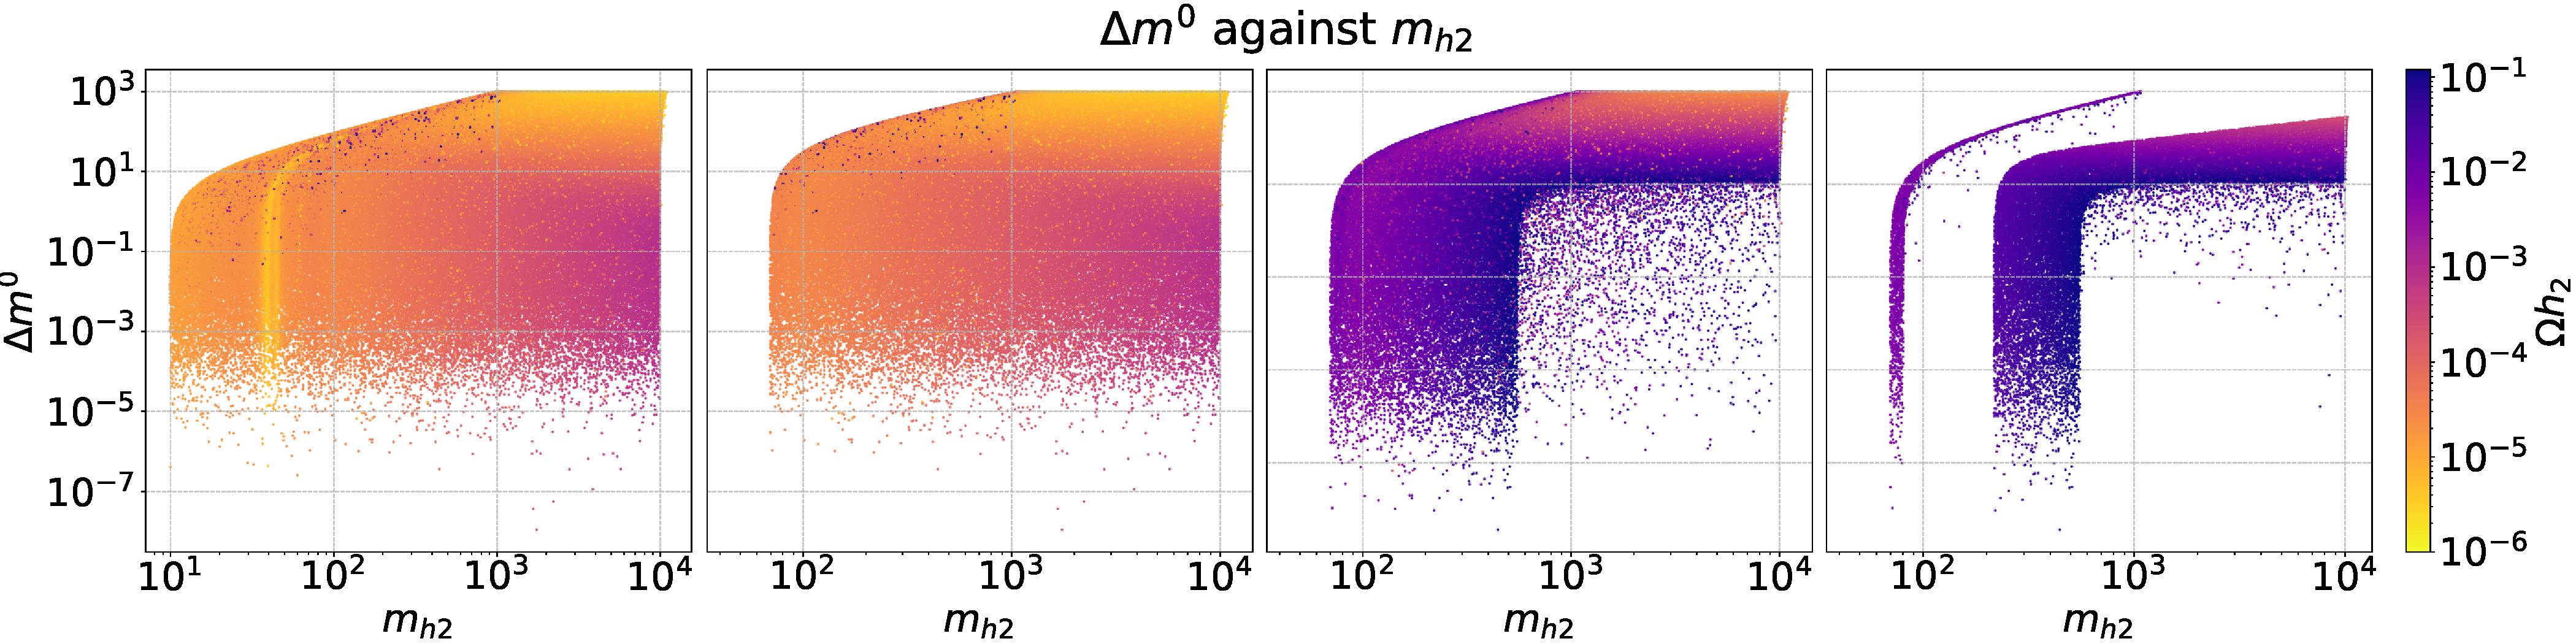
\includegraphics[width=1\columnwidth]{4plot/MD2_DM3.pdf}
    \end{subfigure}

    \begin{subfigure}[b]{\columnwidth}
      \centering
      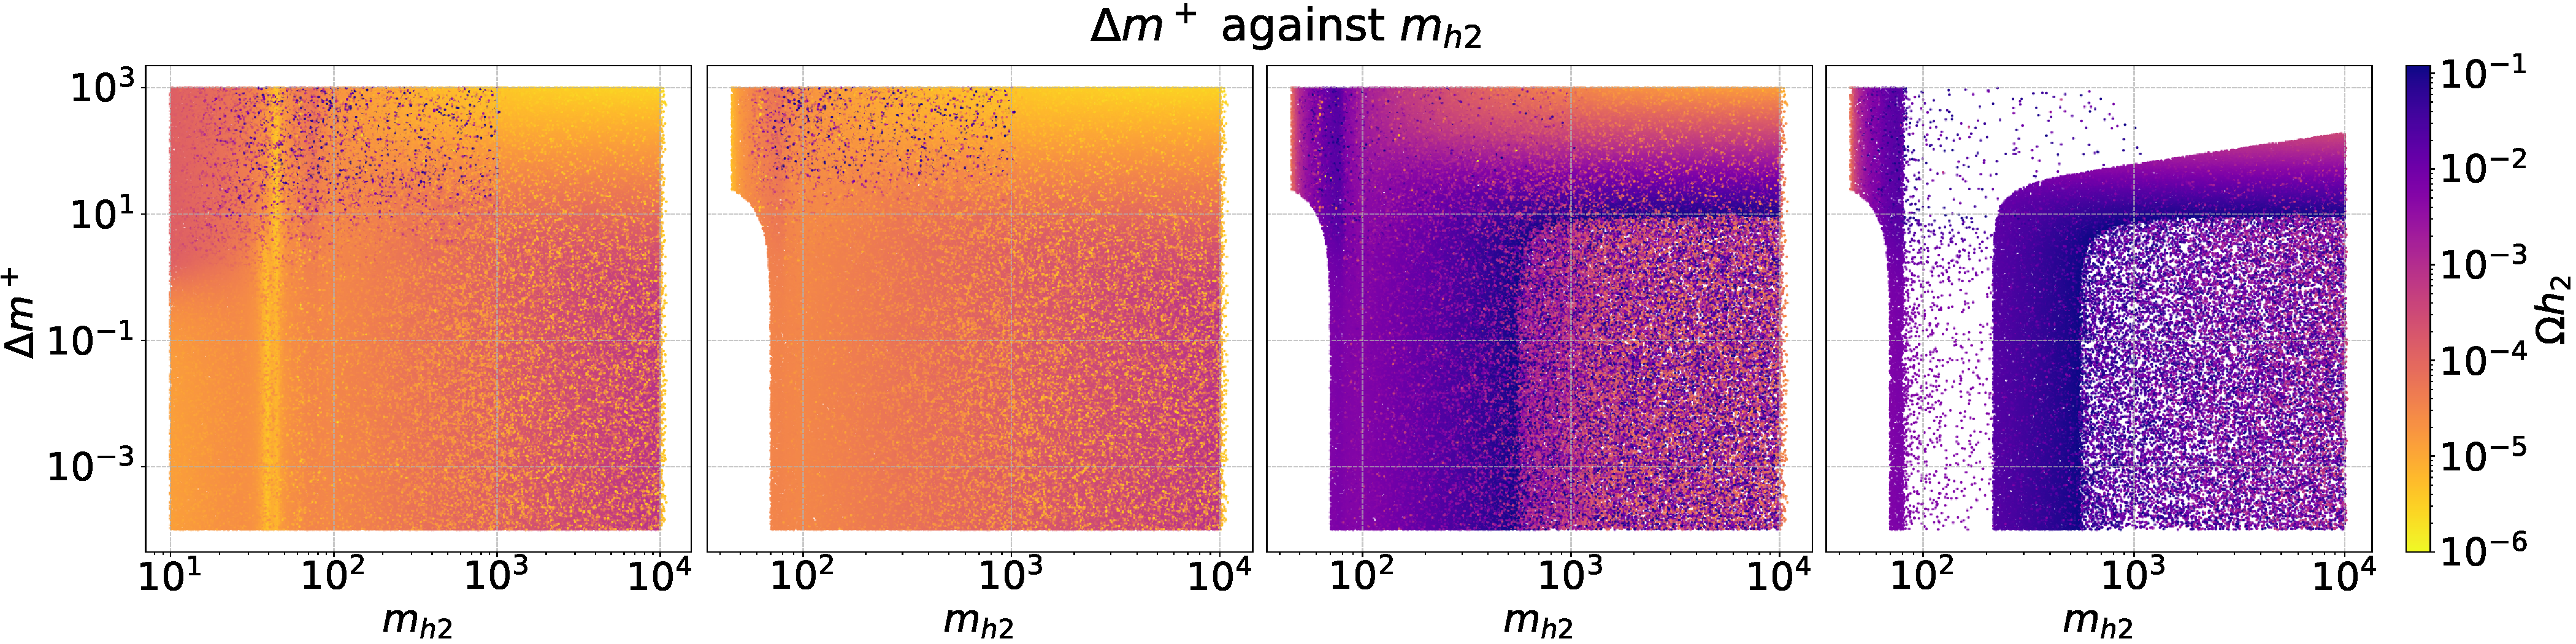
\includegraphics[width=1\columnwidth]{4plot/MD2_DMP.pdf}
    \end{subfigure}
    \caption{Plots with $m_{h2}$ against mass differences.}
\end{figure}

\begin{figure}[H]
    \begin{subfigure}[b]{\columnwidth}
      \centering
      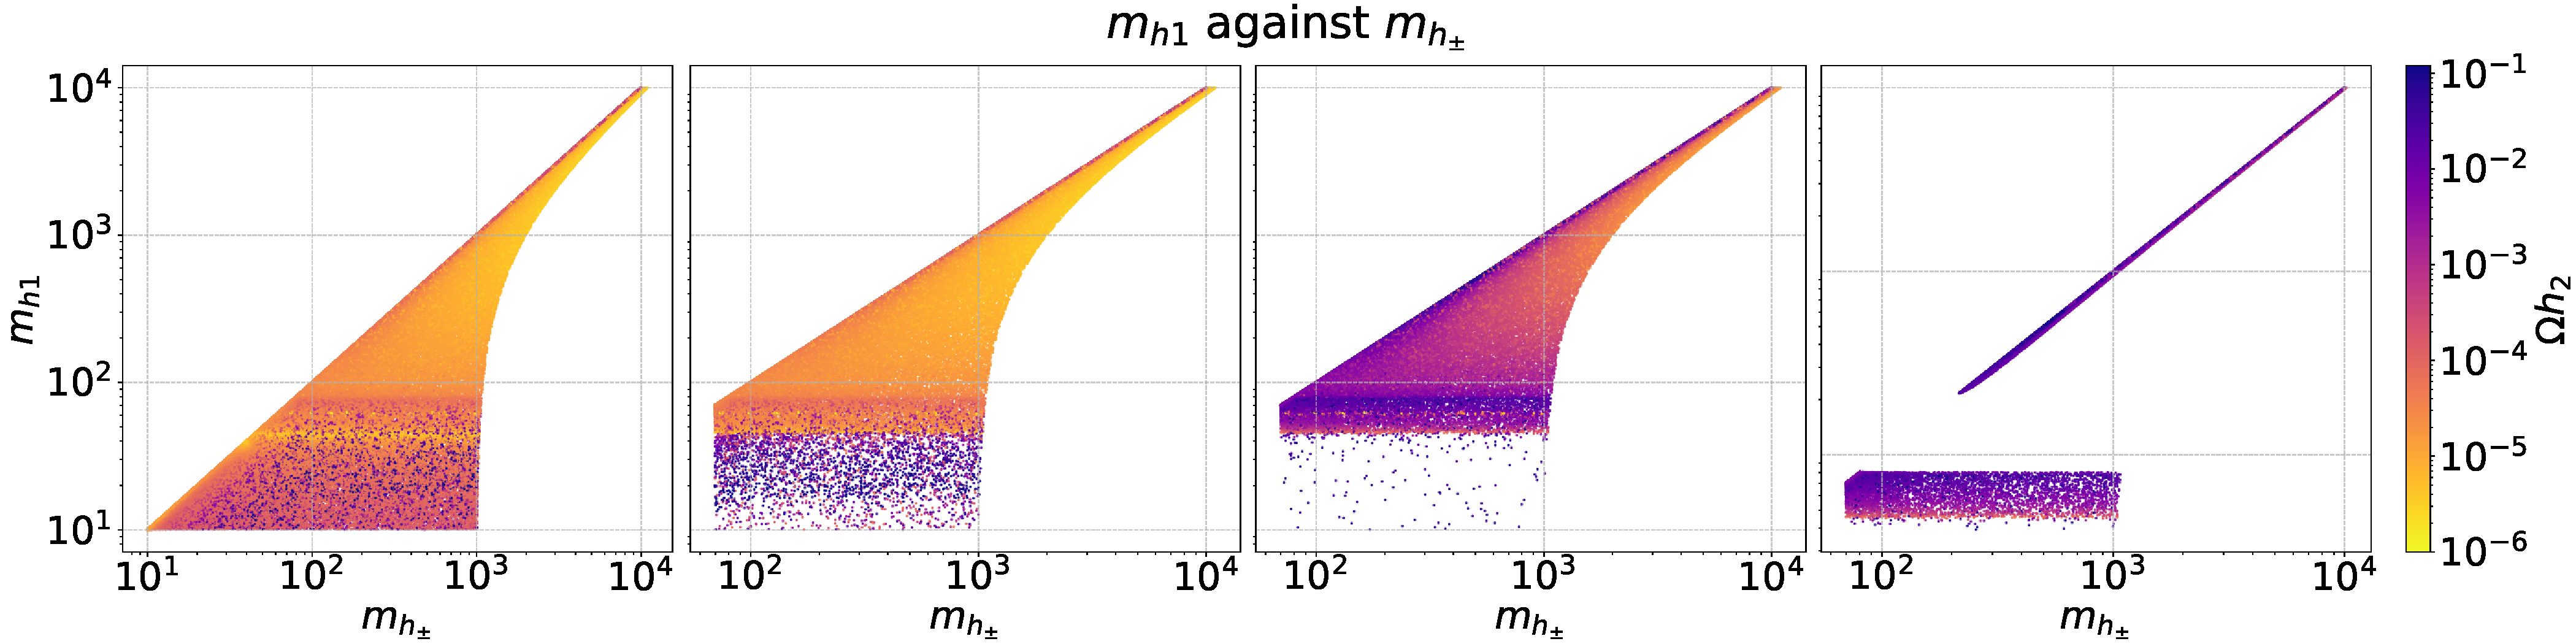
\includegraphics[width=1\columnwidth]{4plot/MDP_MD1.pdf}
    \end{subfigure}

    \begin{subfigure}[b]{\columnwidth}
      \centering
      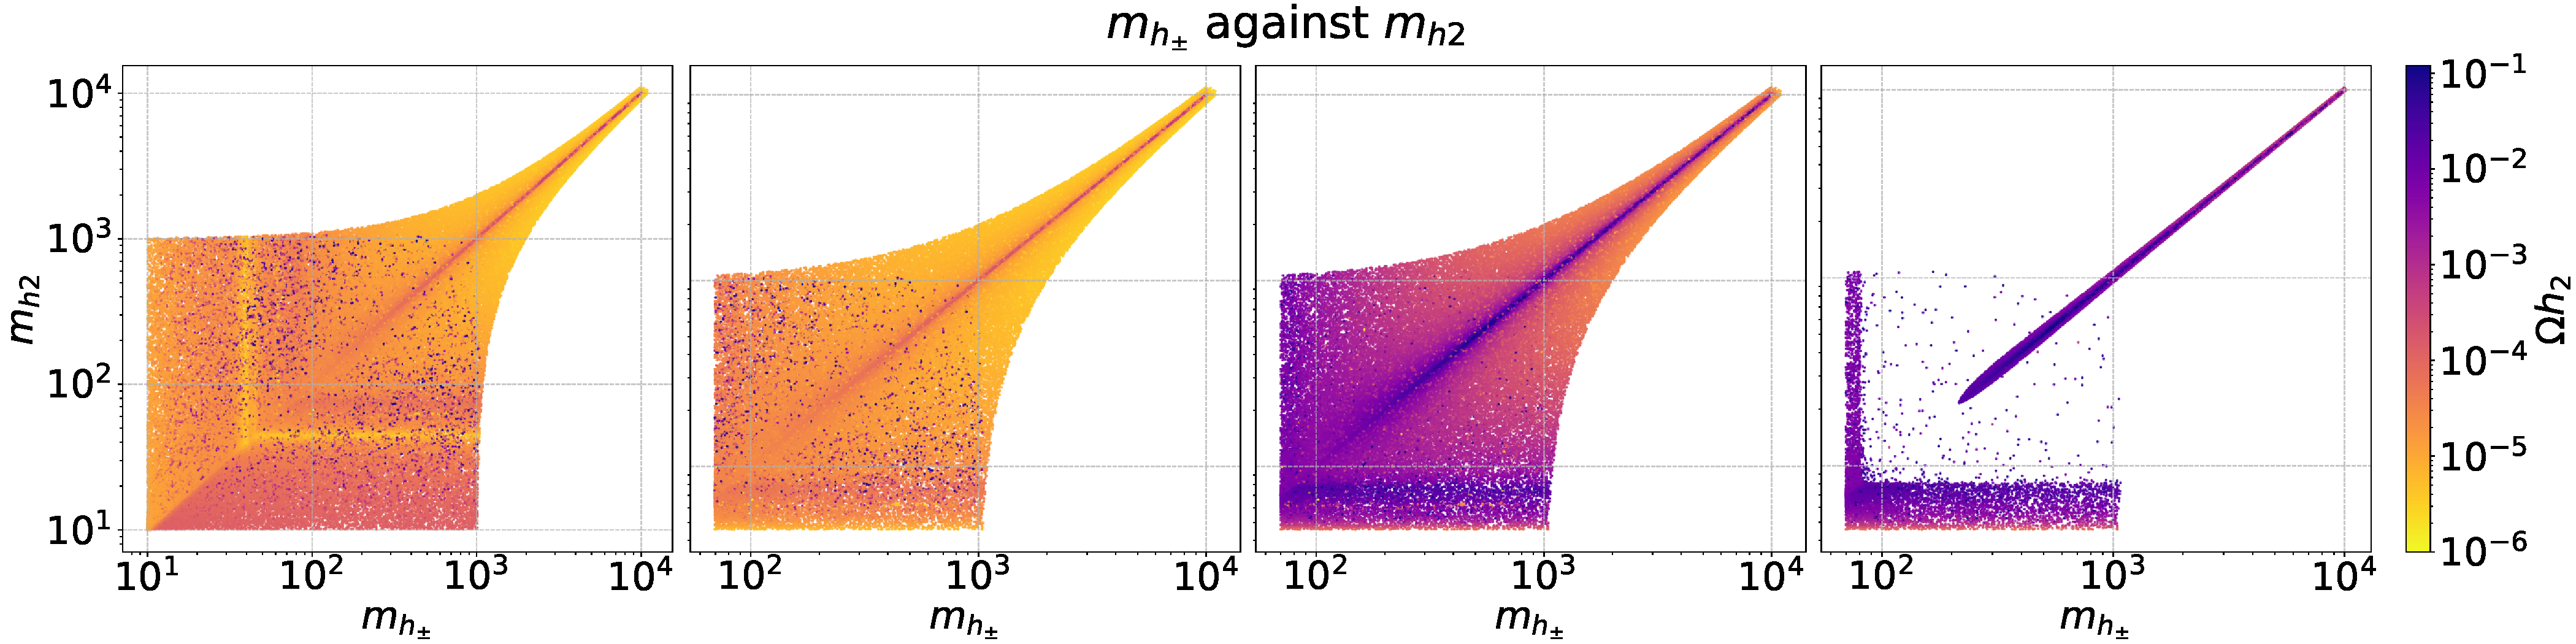
\includegraphics[width=1\columnwidth]{4plot/MDP_MD2.pdf}
    \end{subfigure}
    \caption{Plots of $m_{h_\pm}$ against other masses.}
\end{figure}

\begin{figure}[H]
    \begin{subfigure}[b]{\columnwidth}
      \centering
      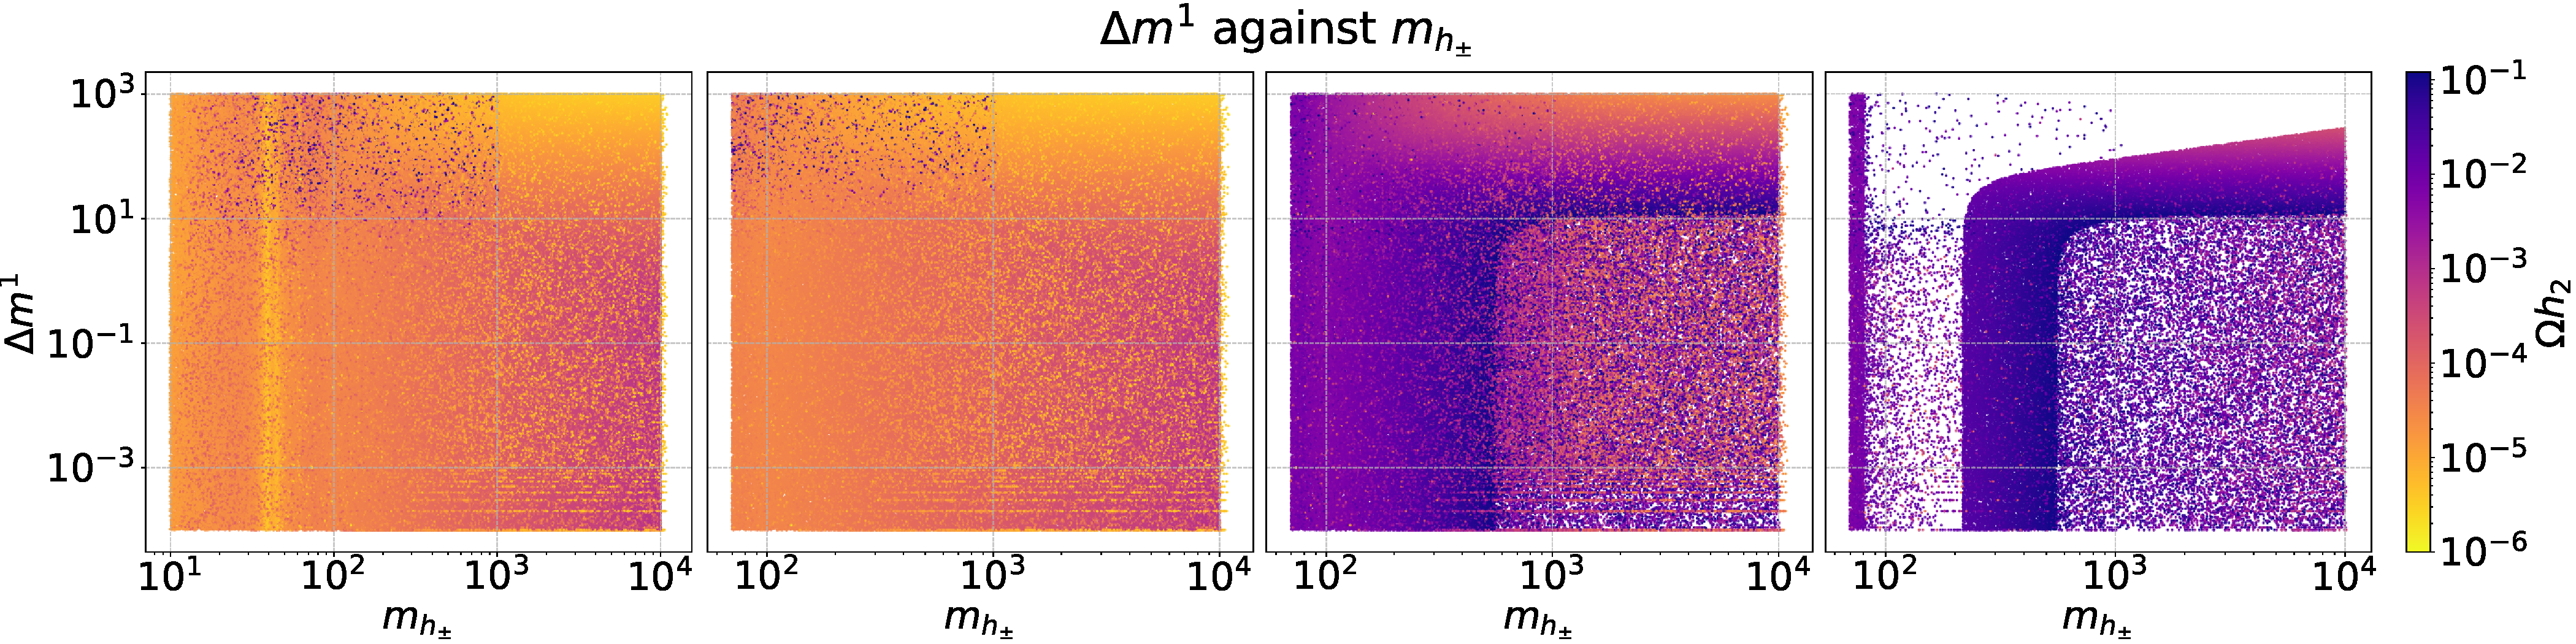
\includegraphics[width=1\columnwidth]{4plot/MDP_DM2.pdf}
    \end{subfigure}
    
    \begin{subfigure}[b]{\columnwidth}
      \centering
      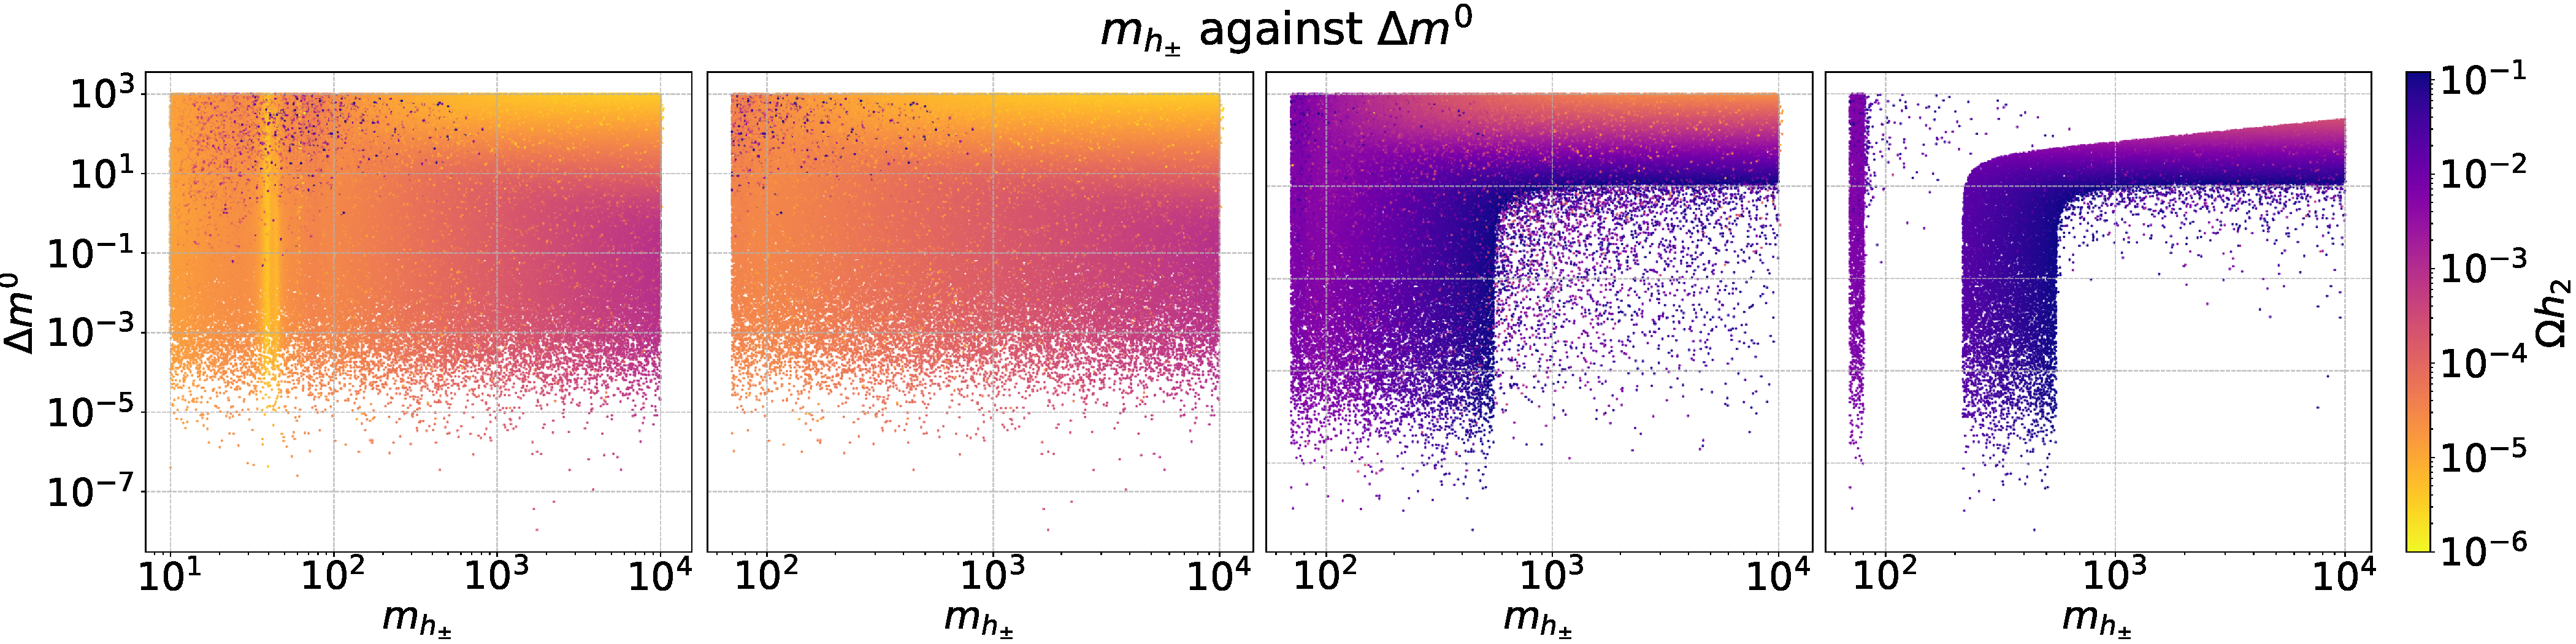
\includegraphics[width=1\columnwidth]{4plot/MDP_DM3.pdf}
    \end{subfigure}

    \begin{subfigure}[b]{\columnwidth}
      \centering
      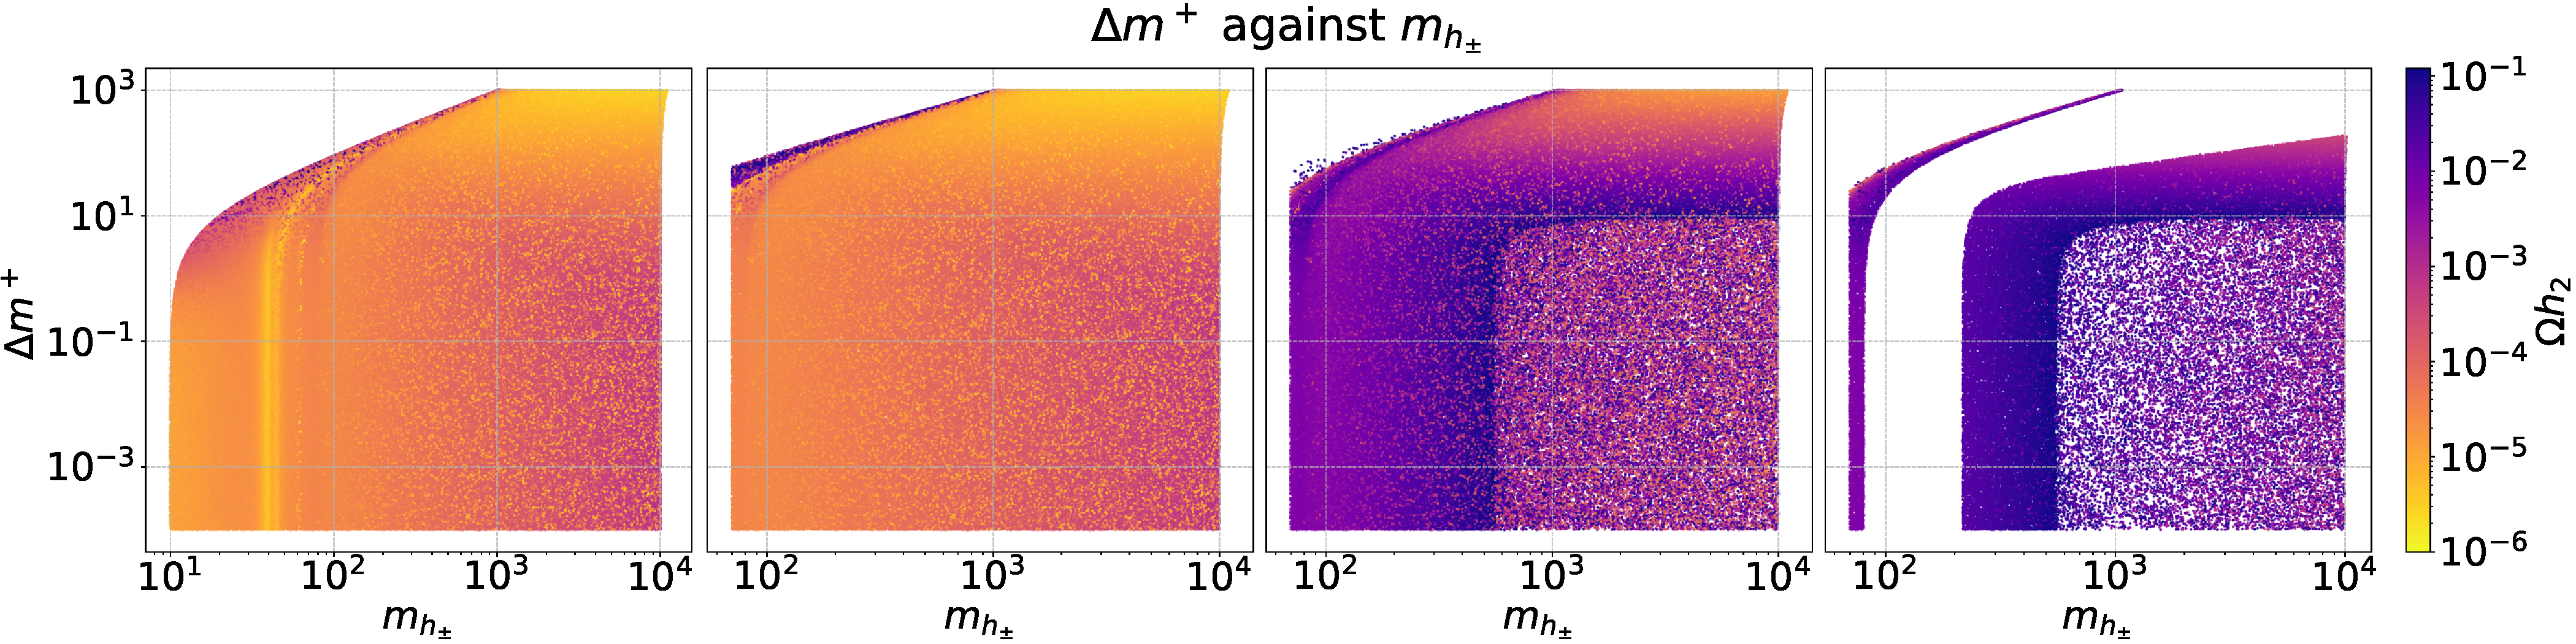
\includegraphics[width=1\columnwidth]{4plot/MDP_DMP.pdf}
    \end{subfigure}
    \caption{Plots with $m_{h_\pm}$ against mass differences.}
\end{figure}

\begin{figure}[H]
    \begin{subfigure}[b]{\columnwidth}
      \centering
      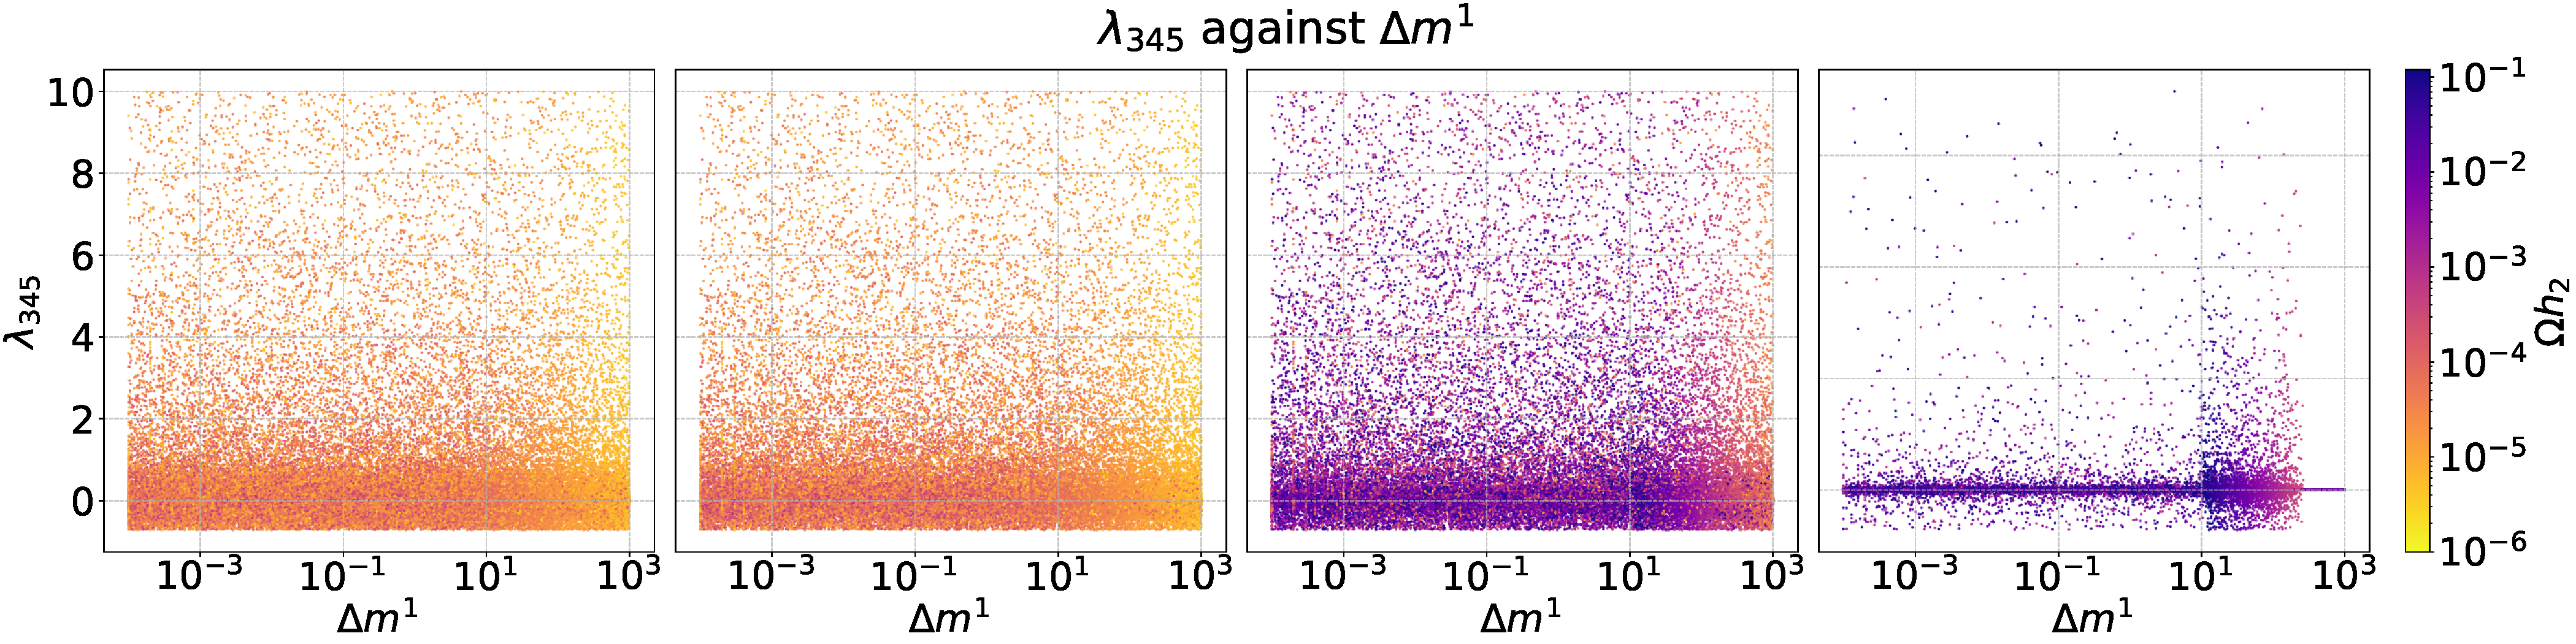
\includegraphics[width=1\columnwidth]{4plot/DM2_l345.pdf}
    \end{subfigure}
    
    \begin{subfigure}[b]{\columnwidth}
      \centering
      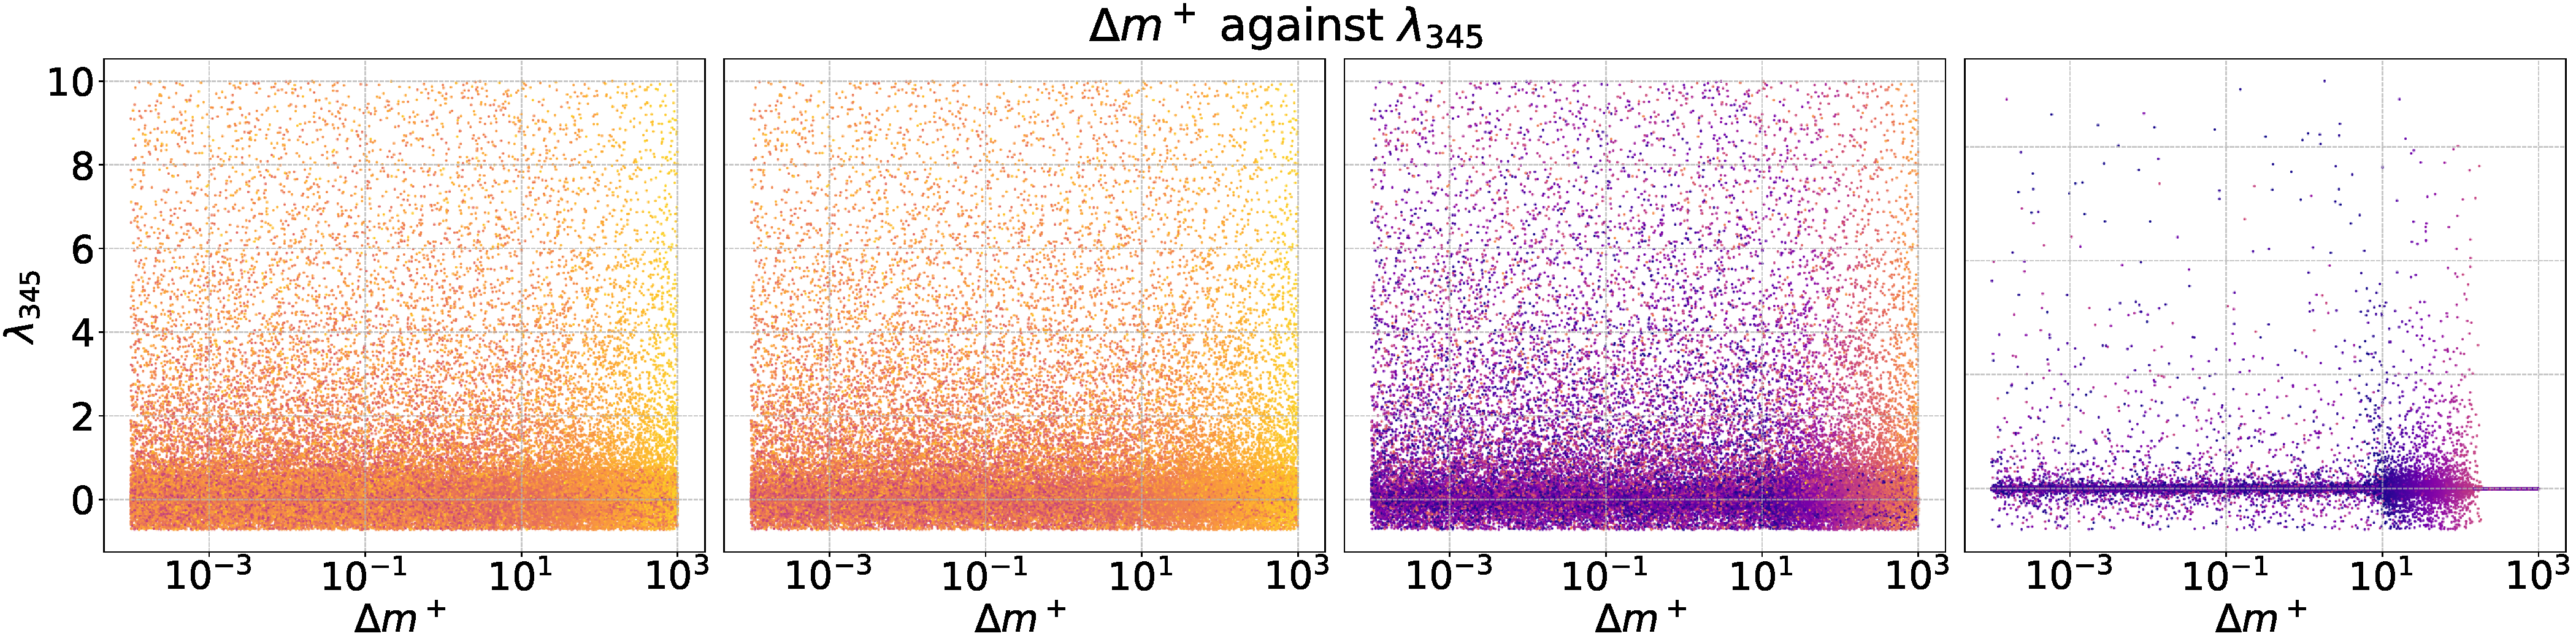
\includegraphics[width=1\columnwidth]{4plot/DMP_l345.pdf}
    \end{subfigure}
    
    \begin{subfigure}[b]{\columnwidth}
      \centering
      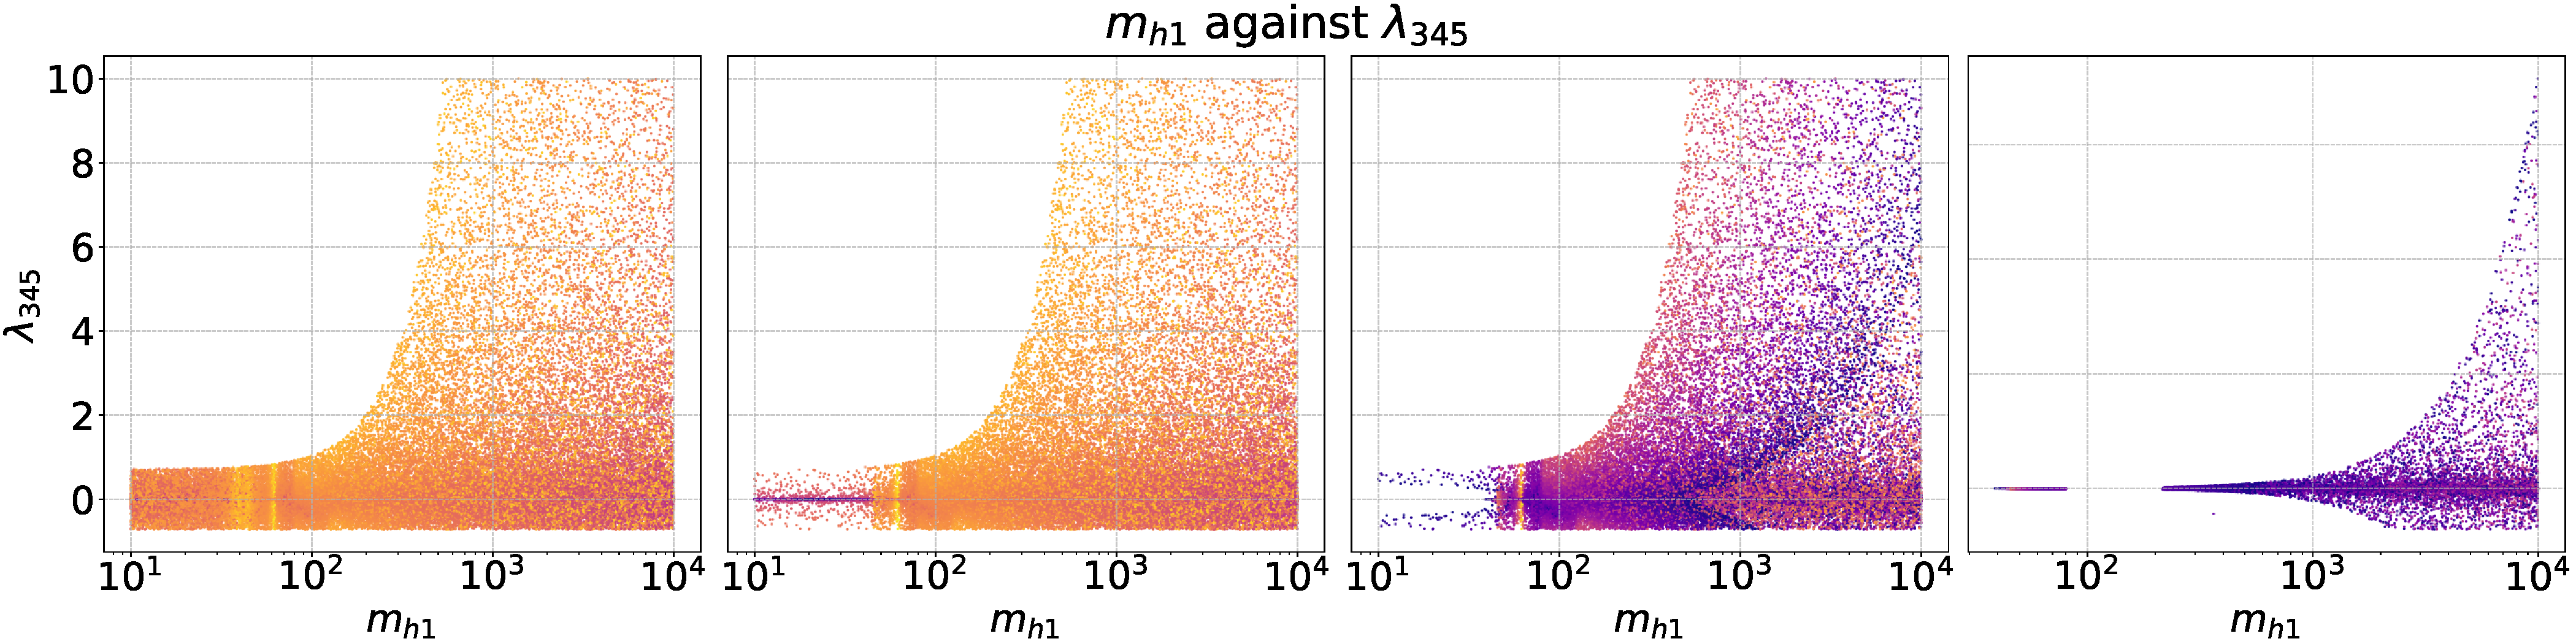
\includegraphics[width=1\columnwidth]{4plot/MD1_l345.pdf}
    \end{subfigure}   
    
    \begin{subfigure}[b]{\columnwidth}
      \centering
      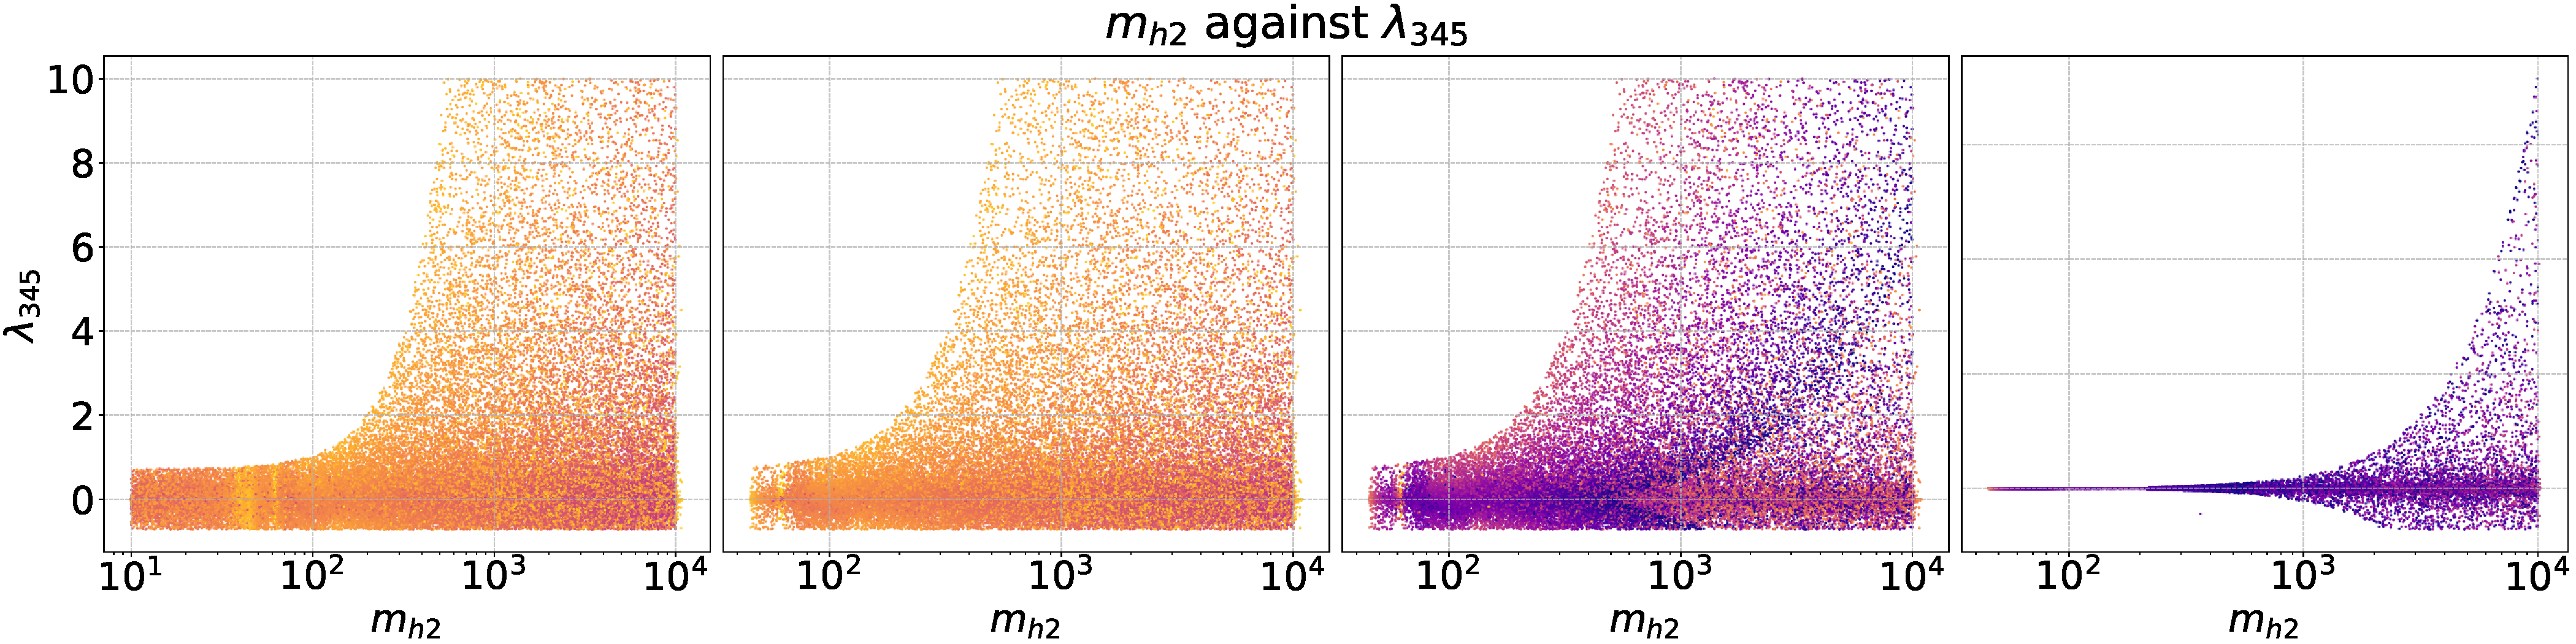
\includegraphics[width=1\columnwidth]{4plot/MD2_l345.pdf}
    \end{subfigure}

    \begin{subfigure}[b]{\columnwidth}
      \centering
      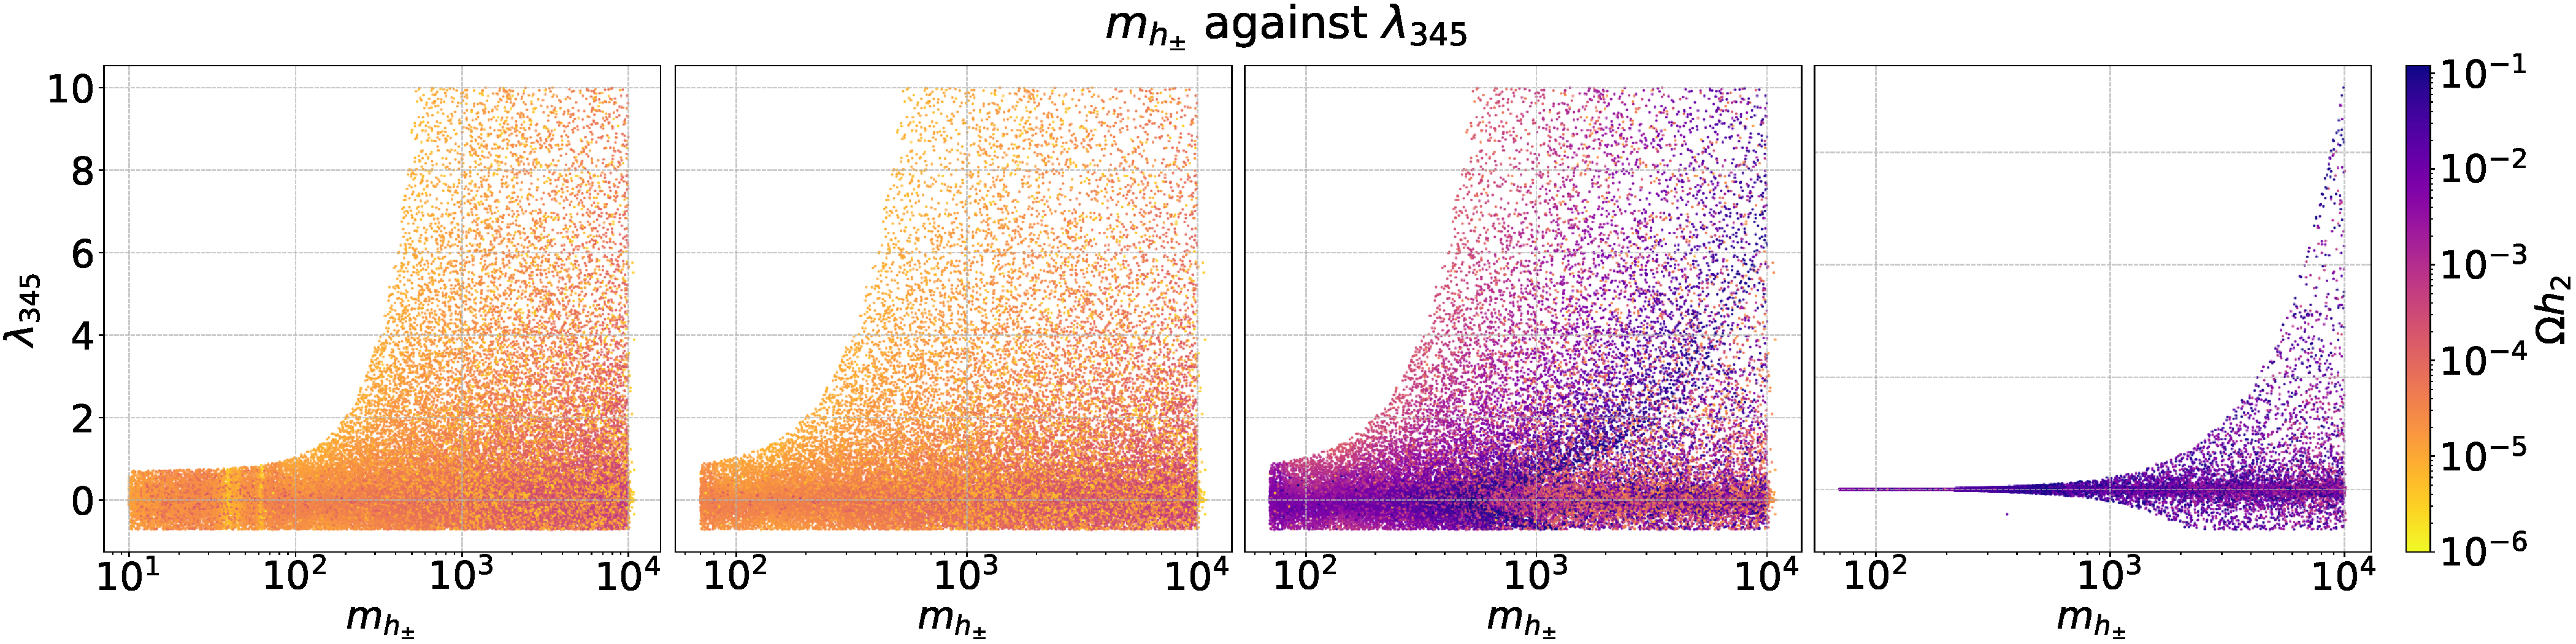
\includegraphics[width=1\columnwidth]{4plot/MDP_l345.pdf}
    \end{subfigure}
\caption{Plots with other parameters against $l_{345}$.}
\end{figure}

\end{document}